% Template for the submittion to:
%   Annals of Mathematical Sciences and Applications [amsa]
%
% Author: In this template, the places where you need to add information
%         (or delete line) are indicated by {???}.  Mostly the information
%         required is obvious, but some explanations are given in lines starting
% Author:
% All other lines should be ignored.  After editing, there should be
% no instances of ??? after this line.

% journal options: amsa
\documentclass[amsa]{ipart}

\usepackage{mymacros}
%\usepackage{citesort}

%\usepackage{amsthm,amsmath}
%\usepackage[numbers,square]{natbib}
%\RequirePackage{hyperref}

% will be filled by editor:
\pubyear{2014}
\volume{0}
\issue{0}
\firstpage{1}
\lastpage{1}
%\arxiv{}

% put your definitions there:
\startlocaldefs
\endlocaldefs

\begin{document}

\begin{frontmatter}

% "Title of the Paper"
\title{Spectral analysis and computation \\
  of effective diffusivities in 
  space-time periodic incompressible flows}
%\thankstext{t1}{Title thanks}
\runtitle{Spectral analysis of space-time periodic flows}

% indicate corresponding author with \corref{}
% \author{\fnms{John} \snm{Smith}\thanksref{t2}\corref{}\ead[label=e1]{smith@foo.com}\ead[label=e2,url]{www.foo.com}}
% \thankstext{t2}{Thanks to somebody}
% \address{line 1\\ line 2\\ \printead{e1}\\ \printead{e2}}

\begin{aug}
\author{\fnms{N. Benjamin} \snm{Murphy,}
  \thanksref{t1,t2,t3}
  \ead[label=e1]{nbmurphy@math.uci.edu}}
\address{University of California at Irvine, Department of Mathematics, 340
Rowland Hall, \\Irvine, CA 92697-3875, USA
\printead{e1}}
%\and
\author{\fnms{Elena} \snm{Cherkaev,}
  \thanksref{t2,t3}
  \ead[label=e2]{elena@math.utah.edu}}
\address{University of Utah, Department of Mathematics, 
155 South 1400 East Room 233, \\Salt Lake City, UT 84112-0090, USA
\printead{e2}}
%\and
\author{\fnms{Jack} \snm{Xin,}
  \thanksref{t1}
  \ead[label=e3]{jxin@math.uci.edu}}
\address{University of California at Irvine, Department of Mathematics, 340
Rowland Hall, \\Irvine, CA 92697-3875, USA
\printead{e3}}
%\and
\author{\fnms{Jingyi} \snm{Zhu,}
  \thanksref{t2,t3}
  \ead[label=e4]{zhu@math.utah.edu}}
\address{University of Utah, Department of Mathematics, 
155 South 1400 East Room 233, \\Salt Lake City, UT 84112-0090, USA
\printead{e4}}
\and
\author{\fnms{Kenneth M.} \snm{Golden}
  \thanksref{t2,t3}
  \ead[label=e5]{golden@math.utah.edu}}
\address{University of Utah, Department of Mathematics, 
155 South 1400 East Room 233, \\Salt Lake City, UT 84112-0090, USA
\printead{e5}}

\thankstext{t1}{NSF Grant DMS-1211179}
\thankstext{t2}{NSF Grant DMS-0940249}
\thankstext{t3}{ONR Grant N00014-12-1086}

\runauthor{Murphy et al.}

\affiliation{University of California, Irvine and University of Utah}

\end{aug}



\begin{abstract}
The enhancement in diffusive transport of passive tracer particles by
incompressible, turbulent flow fields is a challenging problem with
theoretical and practical importance in many areas of science and
engineering, ranging from the transport of mass, heat, and pollutants
in geophysical flows to sea ice dynamics and turbulent combustion. The
long time, large scale behavior of such systems is equivalent to an
enhanced diffusive process with an effective diffusivity tensor
$\Dm^*$. Two different formulations of integral representations for
$\Dm^*$ were developed for the case of \emph{time-independent} fluid
velocity fields, involving spectral measures of \emph{bounded}
self-adjoint operators acting on vector fields and scalar fields,
respectively. Here, we extend both of these approaches to the case of
\emph{space-time periodic} velocity fields, with possibly chaotic
dynamics, providing rigorous integral representations for $\Dm^*$
involving spectral measures of \emph{unbounded} self-adjoint
operators. We prove the different formulations are
equivalent. Their correspondence follows from a one-to-one isometry
between the underlying Hilbert spaces. We also develop a Fourier
method for computing $\Dm^*$, which captures the phenomenon of
residual diffusion related to Lagrangian chaos of a model flow. This
is reflected in the spectral measure by a concentration of mass near
the spectral origin.    
\end{abstract}

\begin{keyword}[class=AMS]
\kwd[Primary ]{47B15,65C60,35C15,\\76B99,76M22,76M50,76R99}
%\kwd{}
%\kwd[; secondary ]{}
\end{keyword}

\begin{keyword}
\kwd{advective diffusion}
\kwd{homogenization}
\kwd{effective diffusivity}
\kwd{spectral measure}
\kwd{integral formula}
\kwd{Fourier method}
\kwd{generalized eigenvalue computation}
\kwd{residual diffusion}
%\kwd{}
\end{keyword}

% history:
% \received{\smonth{1} \syear{0000}}

%\tableofcontents

\end{frontmatter}


\section{Introduction}\label{sec:Introduction}
The long time, large scale motion of diffusing particles or
tracers being advected by an incompressible flow field is equivalent
to an enhanced diffusive process~\cite{Taylor:PRSL:196} with an
effective diffusivity tensor $\Dm^*$. Describing the associated
transport properties is a challenging problem with a broad range of
scientific and engineering applications, such as stellar
convection~\cite{Knobloch:1992ApJ,Press:1981:ApJ,canut98,canut98b,canut00},
turbulent
combustion~\cite{Aslanyan:BF00790149,Bilger:05:10.1016,Tabaczynski:1990:243,Williams:1985:TC:9781611971064,Peters:2000:TC:9780521660822,Xin:2009:Fronts:9780387876832},
and solute transport in porous
media~\cite{Bhattacharya:AAP:1999:951,Bhattacharya:1989:ASD,Whitaker:AIC690130308,Gupta:WRCR3940,Koch:1988:965,Lester:PRL:111.174101,Koch:JFM:7961001}.
Time-dependent flows can have fluid velocity fields with chaotic
dynamics, which gives rise to turbulence that greatly enhances the
mixing, dispersion, and large scale transport of diffusing
scalars. Here we develop a mathematical framework that provides an
analytic representation of $\Dm^*$ for such time-dependent, chaotic
flows. This representation is given in terms of a Stieltjes integral
involving the spectral measure of an \emph{unbounded} self-adjoint
operator. We demonstrate that this approach provides an effective
method for computing $\Dm^*$ for chaotic flows. 


\subsection{Advection enhanced diffusion in the climate system}
\label{sec:AD_in_the_climate}
%
In the climate
system~\cite{Csanady:1973:9789027702609,Griffies:2003:10.1007},
turbulence plays a key role in transporting mass, heat, momentum,
energy, and salt in geophysical
flows~\cite{Moffatt:RPP:621}. Turbulence enhances the dispersion of
atmospheric gases~\cite{Espinosa:MET1292} such as
ozone~\cite{Holton:JGRC2495,Pitari:JGR:1986,Plumb:JAS:1979,Plumb:JAS:1987}
and
pollutants~\cite{Bilger:10.1175,Beychok:1994:9780964458802,Samson:1988:88009978},
as well as atmosphere-ocean transfers of carbon dioxide and other
climatically important trace gas
fluxes~\cite{Zappa:2007:67613,Banerjee:10.1007}.  Longitudinal
dispersion of passive scalars in oceanic flows can be enhanced by
horizontal turbulence due to shearing of tidal currents, wind drift,
or
waves~\cite{Young:JPO:1982:515,Kullenberg:1972:TUS1529,Bowden:JFM:1965}.   
Chaotic motion of 
time-dependent fluid velocity fields cause instabilities in large
scale ocean currents, generating geostrophic
eddies~\cite{Ferrari:JPO:1501} which dominate the kinetic energy of
the ocean~\cite{Ferrari:ARFM:253}. Geostrophic
eddies greatly enhance~\cite{Ferrari:JPO:1501} the meridional mixing
of heat, carbon and other climatically important tracers, typically
more than one order of magnitude greater than the mean flow of the
ocean~\cite{Souza:OS:317}. Eddies also impact heat and salt budgets
through lateral fluxes and can extend the area of high biological
productivity offshore by both eddy chlorophyll advection and eddy
nutrient pumping~\cite{Chaigneau:JGR:C11025}. 

In sea ice dynamics,
where the ice cover couples the atmosphere to the polar
oceans \cite{Washington:1986:9780935702521}, the transport of sea 
ice can also be enhanced by eddie
fluxes and large scale coherent structures in the ocean
\cite{Watanabe:2009JPO4010,Lukovich:AG:2015}. 
In sea ice thermodynamics, the temperature field of the 
atmosphere is coupled to the temperature field of the ocean through
sea ice, which is a composite of pure ice with brine inclusions
whose volume fraction and connectedness depend strongly
on temperature.
Convective brine flow through the porous
microstructure can enhance thermal transport through the sea ice layer
\cite{Lytle:JGR-8853,Worster:PTRSA:2015,Liu:2015}.




Both numerical and observational studies of scalar transport have
suggested that tracers are advected over large scales by a fluid
velocity field that is different from the mean
flow~\cite{Pavliotis:PHD_Thesis}. This suggests that the effective
diffusivity tensor $\Dm^*$ should be spatially and possibly also
temporally inhomogeneous~\cite{Pavliotis:PHD_Thesis}. The mixing of
eddy fluxes is typically non-divergent and unable to affect the
evolution of the mean flow~\cite{Middleton:JPO:5840223}, and do not
alter the tracer moments~\cite{Griffies:JPO:1998}. In this sense, the
mixing is non-dissipative, reversible, and sometimes referred to as
stirring~\cite{Eckart:JMR:1948,Griffies:JPO:1998}. It has been noted
in various geophysical contexts~\cite{Plumb:JAS:1979,Plumb:JAS:1987}
that eddy-induced skew-diffusive tracer fluxes directed normal to
the tracer gradient~\cite{Middleton:JPO:5840223}] are generally
equivalent to \emph{antisymmetric} components in the effective
diffusivity tensor $\Dm^*$, while the \emph{symmetric} part of $\Dm^*$
represents irreversible diffusive
effects~\cite{Redi:JPO:1982:1154,Solomon:OGR:1971:233,Griffies:JPO:1998}
directed down the tracer gradient.  Motivated by these observations,
we provide in the ensuing sections analytic representations for both
the \emph{symmetric and antisymmetric} components of $\Dm^*$. 



\subsection{Mathematical characterization of effective diffusivity}
%
Due to the computational intensity of detailed climate
models~\cite{Griffies:2003:10.1007,Washington:1986:9780935702521,Neelin:2010:CCCM},
a coarse resolution is necessary in numerical simulations and
\emph{parameterization} is used to help resolve sub-grid
processes, such as turbulent 
entrainment-mixing processes in clouds~\cite{Lu:JGR:D50094},
atmospheric boundary layer turbulence~\cite{Bretherton:JOC:5655449},
atmosphere-surface exchange over the
sea~\cite{Fairall:1996:JGRC6562} and sea
ice~\cite{Sorensen:TC:2014,Andreas:2010:QJ618,Andreas:JH:2010,Vihma:2014:9923},
and eddies in the ocean~\cite{McDougall:2001:book,Gent:JPO:1995}. In
this way, only the effective or averaged behavior of these sub-grid
processes are included in the models. Here, we study the effective
behavior of advection enhanced diffusion by time-dependent fluid
velocity fields, with possibly chaotic dynamics, which gives rise to
such a parameterization, namely, the effective diffusivity tensor
$\Dm^*$ of the flow. 



In recent decades, a broad range of mathematical techniques have been
developed
%
%Advective-Diffusion:
%\cite{McLaughlin:SIAM_JAM:780,Biferale:PF:2725,Fannjiang:1994:SIAM_JAM:333,Novikov:2005:CPAM:867,Pavliotis:PHD_Thesis}
%Porous Media:
%\cite{Mauri:1991:3:743,Clark:1998:364,Hornung:1997:9780387947860}
%Books:
%\cite{Bensoussan:Book:1978,Holmes:1995:94481954}
%Stochastic DEs:
%\cite{Pavliotis:CMS:2007:507,Fannjiang:1997:1033}
%Reaction-Advection-Diffusion:
%\cite{Majda:Kramer:1999:book,Majda:1994:10.1088}
%
which reduce the analysis of enhanced diffusive transport by complex
fluid velocity fields with rapidly varying structures in both space
and time, to 
solving averaged or \emph{homogenized} equations that do not have
rapidly varying data, and involve an effective
parameter~\cite{Papanicolaou:1981:36:8,McLaughlin:SIAM_JAM:780,Bensoussan:Book:1978,Biferale:PF:2725,Fannjiang:1994:SIAM_JAM:333,Novikov:2005:CPAM:867,Fannjiang:1997:1033,Mauri:1991:3:743,Pavliotis:PHD_Thesis,Pavliotis:CMS:2007:507,Clark:1998:364,Holmes:1995:94481954,Hornung:1997:9780387947860,Majda:Kramer:1999:book,Majda:1994:10.1088,Xin:2009:Fronts:9780387876832}. Motivated
by~\cite{Papanicolaou:RF-835}, it was
shown~\cite{McLaughlin:SIAM_JAM:780} that the homogenized behavior of
the advection-diffusion equation with a random, time-independent,
incompressible, mean-zero fluid velocity field, is given by an
inhomogeneous diffusion equation involving the symmetric part
of an effective diffusivity tensor $\Dm^*$. Moreover, a rigorous
representation of $\Dm^*$ was given in terms of an auxiliary ``cell
problem'' involving a curl-free random
field~\cite{McLaughlin:SIAM_JAM:780}. We stress that the effective
diffusivity tensor $\Dm^*$ is not symmetric in general. However, only
its symmetric part appears in the homogenized equation for \emph{this} 
formulation of the effective transport properties of advection
enhanced diffusion~\cite{McLaughlin:SIAM_JAM:780}.    



The incompressibility condition of the time-independent fluid velocity
field was used~\cite{Avellaneda:PRL-753,Avellaneda:CMP-339} to
transform the cell problem in~\cite{McLaughlin:SIAM_JAM:780} into the
quasi-static limit of Maxwell's
equations~\cite{Jackson-1999,Golden:CMP-473}, which describe the
transport properties of an electromagnetic wave in a composite
material~\cite{Milton:2002:TC}. The analytic continuation method for
representing transport in composites~\cite{Golden:CMP-473} provides
Stieltjes integral representations for the bulk transport coefficients
of composite media, such as electrical conductivity and permittivity,
magnetic permeability, and thermal
conductivity~\cite{Milton:2002:TC}. This method is based on the
spectral theorem~\cite{Stone:64,Reed-1980} and a resolvent formula
for, say, the electric field, involving a random self-adjoint
operator~\cite{Golden:CMP-473,Murphy:JMP:063506} or
matrix~\cite{Murphy:2015:CMS:13:4:825}. Based on the analytic
continuation method~\cite{Golden:CMP-473}, 
the cell problem for the advection diffusion equation was transformed
into a resolvent formula involving a 
\emph{bounded} self-adjoint operator, acting on the Hilbert
space of curl-free random vector
fields~\cite{Avellaneda:PRL-753,Avellaneda:CMP-339}. This, in turn,     
led to a Stieltjes integral representation for the symmetric part of
the effective diffusivity tensor $\Dm^*$, involving the P{\'e}clet
number $\Pen$ of the flow and a \emph{spectral measure} $\bmu$ of the
operator~\cite{Avellaneda:PRL-753,Avellaneda:CMP-339}. A key feature
of the method is that parameter information in $\Pen$ is 
\emph{separated} from the complicated geometry of the time-independent
flow, which is encoded in the measure $\bmu$. This property led to
rigorous bounds~\cite{Avellaneda:CMP-339} for the diagonal components
of $\Dm^*$. Bounds for $\Dm^*$ can also be obtained using variational 
methods~\cite{Avellaneda:CMP-339,Fannjiang:1994:SIAM_JAM:333,Novikov:2005:CPAM:867,Fannjiang:1997:1033}.  



The mathematical framework developed in~\cite{McLaughlin:SIAM_JAM:780}
was also
adapted~\cite{Pavliotis:PHD_Thesis,McLaughlin:Forest:PF:1999:880,Majda:Kramer:1999:book} 
to the case of a periodic, 
time-dependent, incompressible fluid velocity field with \emph{non-zero}
mean. The velocity field was modeled as a superposition of a
large-scale mean flow with small-scale periodically oscillating 
fluctuations. It was shown~\cite{Pavliotis:PHD_Thesis} that, depending
on the strength of the fluctuations relative to the mean flow, the
effective diffusivity tensor $\Dm^*$ can be constant or a function of
both space and time. When $\Dm^*$ is
constant, only its symmetric part 
appears in the homogenized equation as an enhancement in the
diffusivity. However, when $\Dm^*$ is a function of space and time,
its antisymmetric part also plays a key role in the homogenized
equation. In particular, the symmetric part of $\Dm^*$ appears as an
enhancement in the diffusivity, while both the symmetric and
antisymmetric parts of $\Dm^*$ contribute to an effective drift in the
homogenized equation. The effective drift due to the antisymmetric
part is purely sinusoidal, thus
divergence-free~\cite{Pavliotis:PHD_Thesis}. This is consistent with
what has been observed in geophysical flows in the climate system, as
discussed in the final paragraph of
\secref{sec:AD_in_the_climate}. 


Based on~\cite{Bhattacharya:AAP:1999:951}, the cell problem discussed
in~\cite{Pavliotis:PHD_Thesis} was transformed into a resolvent formula
involving a self-adjoint operator, acting on the Sobolev
space~\cite{McOwen:2003:PDE,Folland:95:PDEs} of spatially periodic scalar
fields, which is also a Hilbert space. In the case where the mean flow
and periodic fluctuations are time-independent, the
self-adjoint operator is compact~\cite{Bhattacharya:AAP:1999:951},
hence \emph{bounded}~\cite{Stakgold:BVP:2000}. This led to a
discrete Stieltjes integral representation for the
antisymmetric part of $\Dm^*$, involving the P{\'e}clet number of the
steady flow and a spectral measure of the operator.    



The incompressibility of the fluid velocity field was a central
property of the mathematical frameworks described above. However,
in~\cite{McLaughlin:Forest:PF:1999:880}, these results were extended
to weakly compressible, anelastic, stratified, time-independent, fluid
velocity fields. Homogenization of the convection-reaction-diffusion
equation with compressible velocity field was treated
in~\cite{Papanicolaou:1995:Diff_Rand_Media}.  


\subsection{Summary of Results}
%
Here, we generalize both of the approaches described
in~\cite{Avellaneda:PRL-753,Avellaneda:CMP-339}
and~\cite{Pavliotis:PHD_Thesis} to the case of an incompressible,
periodic, \emph{time-dependent} fluid velocity field, allowing for
chaotic dynamics. In particular, for each approach, we provide Stieltjes
integral representations for both the symmetric and antisymmetric
parts of the effective diffusivity tensor $\Dm^*$, involving a
spectral measure of a self-adjoint operator. In this time-dependent
setting, the underlying operator becomes \emph{unbounded}. The
spectral theory of unbounded operators is more subtle and technically
challenging than the spectral theory of bounded operators, since the
domain of an unbounded operator and its adjoint plays a central role
in the 
spectral characterization of the operator. Neglecting such important 
mathematical details, the Stieltjes integral representation for
$\Dm^*$ given in~\cite{Avellaneda:PRL-753,Avellaneda:CMP-339} was
extended to the time-dependent setting
in~\cite{Avellaneda:PRE:3249}. Here, we provide a mathematically 
rigorous formulation of Stieltjes integral representations for $\Dm^*$
in the time-dependent, unbounded operator setting. We prove that the
two approaches described
in~\cite{Avellaneda:PRL-753,Avellaneda:CMP-339}
and~\cite{Pavliotis:PHD_Thesis} are equivalent in this setting, and
that their correspondence follows from a one-to-one isometry between
the underlying Hilbert spaces. We also establish a direct
correspondence between the effective parameter problem for $\Dm^*$ and
the effective parameter problem arising in the analytic continuation
method for composite media.  






Analytical calculations of the spectral measure underlying the
effective diffusivity tensor $\Dm^*$ have been obtained
only for a handful of simple models of periodic fluid velocity
fields to date such as shear flows. We develop a 
Fourier method for the computation of $\Dm^*$. In particular, we 
compute the effective properties for the following space-time periodic
flow in two spatial dimensions, with $\vecx=(x,y)$,
%
\begin{align}\label{eq:tdcell}
\vecu (t,\vecx)=(\cos{y},\cos{x}) + \theta\cos{t}\;(\sin{y},\sin{x}),
\quad
\theta \in (0,1].
\end{align}
%
The steady part $(\cos{y}, \cos{x})$ of the flow is subject to a
time-periodic perturbation that gives rise to a transition to
Lagrangian chaos for $\theta>0$~\cite{Biferale:PF:2725,ZCX_2015}. In the
advection dominated regime, we shall compare our computations of the
effective diffusivity for the steady $\theta=0$ and dynamic $\theta=1$ settings.  



The rest of the paper is organized as follows. In
\secref{sec:Eff_Trans} the theory of homogenization for the
advection-diffusion equation for space-time periodic flows is
reviewed. Novel Stieltjes integral representations for the effective
diffusivity tensor are also obtained for a large class of fluid
velocity fields, involving a spectral measure of an \emph{unbounded}
self-adjoint operator. In \secref{sec:Fourier_Methods} we use Fourier
methods to transform the eigenvalue problem for the operator into an
infinite set of algebraic equations. This provides a rigorous
mathematical foundation for the computation of effective diffusivities
for such flows. This framework is employed in \secref{sec:Num_Results}
to compute the discrete component of the spectral measure associated
with the fluid velocity field in \eqref{eq:tdcell} for time-independent
flow $\theta=0$ and time-dependent flow $\theta=1$. Our computations highlight
that the behavior of the measure near the spectral origin governs the
behavior of the effective diffusivity in the advection dominated
regime of small molecular diffusion. In particular, we demonstrate
that for $\theta=0$ there is a \emph{spectral gap} in the measure near a
limit point at the spectral origin, giving rise to the known vanishing
asymptotic behavior of 2D cell
flows~\cite{Fannjiang:1994:SIAM_JAM:333,Novikov:2005:CPAM:867}. However in the time
dependent setting, a strong concentration of measure mass
near the spectral origin gives rise to the phenomenon of residual
diffusivity in the limit of vanishing molecular diffusion.


Technical background information and proofs of the key results of the
paper are deffered to the appendices. The spectral theory of unbounded
self-adjoint operators in Hilbert space is reviewed in 
\appref{app:Spectral_Theory} and \appref{app:Time_Derivative}. Two
mathematical formulations of the effective parameter problem for
advection enhanced diffusion are presented in
\appref{app:Hilbert_Resolvent_Integral_Reps}, leading to novel
integral representations for the symmetric and antisymmetric
components of the effective diffusivity tensor. In
\appref{app:Isometric_Correspondence} we use powerful methods of
functional analysis to prove that the two approaches are equivalent,
which follows from a one-to-one isometry between the associated
Hilbert spaces. In \appref{app:Eig_Funct_Exp} we derive an explicit 
formula for the discrete component of the spectral measure, which is
employed in our numerical computations.





\section{Effective transport by
  advective-diffusion} \label{sec:Eff_Trans}    
%
The density $\phi$ of a cloud of passive tracer particles diffusing along
with molecular diffusivity $\varepsilon$ and being advected by an incompressible
velocity field $\vecu$ satisfies the advection-diffusion equation
%
\begin{align}\label{eq:ADE}
  \partial_t\phi(t,\vecx)
    =\vecu (t,\vecx)\cdot\bnabla \phi(t,\vecx)+\varepsilon\Delta \phi(t,\vecx),
  \quad
  \phi(0,\vecx)=\phi_0(\vecx),  
  % \quad
%   t>0,
%   \quad
%   \vecx\in\mathbb{R}^d.
\end{align}
%
for $t>0$ and $\vecx\in\mathbb{R}^d$.
Here, the initial density $\phi_0(\vecx)$ and the fluid velocity field
$\vecu$ are assumed given, and $\vecu$ satisfies $\bnabla\cdot\vecu=0$.
In equation~\eqref{eq:ADE}, the molecular diffusion constant $\varepsilon>0$,
$d$ is the spatial dimension of the 
system, $\partial_t$ denotes partial differentiation with respect to time
$t$, and $\Delta=\bnabla\cdot\bnabla =\nabla^2$ is the Laplacian. Moreover, 
$\vecpsi\cdot\vecvarphi=\vecpsi^{\,T}\overline{\vecvarphi}$,
$\vecpsi^{\,T}$ denotes transposition of the vector $\vecpsi$, and
$\overline{\vecvarphi}$ denotes component-wise complex conjugation,
with $\vecpsi\cdot\vecpsi=|\vecpsi|^2$. Later, we will extensively use this
form of the dot product over complex fields, with built in complex
conjugation. However, we stress that 
all quantities considered in this section are \emph{real-valued}.




We consider enhanced diffusive transport by a periodic fluid velocity
field and non-dimensionalize equation~\eqref{eq:ADE} as follows. Let
$\ell$ and $T$ be typical length and time scales associated with the
problem of interest. Mapping to the non-dimensional variables
$t\mapsto t/T$ and $\vecx\mapsto \vecx/\ell$,
one finds that $\phi$ satisfies the advection-diffusion equation
in~\eqref{eq:ADE} with a non-dimensional molecular diffusivity 
$\varepsilon\mapsto T\,\varepsilon/\ell^{\,2}$ and velocity field $\vecu\mapsto T\,\vecu /\ell$. There are
several different non-dimensionalizations possible 
for the advection-diffusion equation. A detailed discussion of 
various non-dimensionalizations involving the Strouhal number, the
P{\'e}clet number, and the periodic P{\'e}clet number is given
in~\cite{McLaughlin:Forest:PF:1999:880,Majda:Kramer:1999:book}.  Here,
we focus on the long time, large scale transport characteristics of
equation~\eqref{eq:ADE} as a function of $\varepsilon$. To this end, we simply
take $T$ to be the temporal periodicity of the velocity field $\vecu$
and assume that the spatial periodicity of $\vecu$ is $\ell$ in all
spatial dimensions, i.e., 
%
\begin{align}\label{eq:Periodic_u}
  \vecu(t+T,\vecx)=\vecu(t,\vecx), \qquad
  \vecu(t,\vecx+\ell\,\vece_j)=\vecu(t,\vecx), \quad
  j=1,\ldots,d,
\end{align}
%
where $\vece_j$ is a standard basis vector in the $j$th direction. 



\subsection{Mean-zero flow}\label{sec:Mean_zero_flow}
%
In this section we will discuss the effective transport properties of
advection enhanced diffusion, as described by the advection diffusion
equation in~\eqref{eq:ADE}. We will assume in this section that the
fluid velocity field is mean-zero. The effects of a large-scale mean
flow will be discussed in \secref{sec:Mean_Flow}. 




The long time, large scale dispersion of diffusing tracer particles
being advected by an incompressible fluid velocity field is equivalent
to an enhanced diffusive process~\cite{Taylor:PRSL:196} with an
effective diffusivity tensor $\Dm^*$. In recent decades, methods of
homogenization
theory~\cite{McLaughlin:SIAM_JAM:780,Fannjiang:1994:SIAM_JAM:333,Novikov:2005:CPAM:867,Majda:Kramer:1999:book}
have been used to provide an explicit representation for
$\Dm^*$. In particular, these methods have demonstrated that the
averaged or \emph{homogenized} behavior of the advection-diffusion
equation in~\eqref{eq:ADE}, with space-time periodic velocity field
$\vecu$, is determined by a diffusion equation
involving an averaged scalar density $\bar{\phi}$ and an
%(constant)
effective diffusivity tensor
$\Dm^*$~\cite{Majda:Kramer:1999:book}       
%
\begin{align}\label{eq:phi_bar}
 \partial_t\bar{\phi}(t,\vecx)=\bnabla\cdot[\Dm^*\bnabla \bar{\phi}(t,\vecx)], \quad
  \bar{\phi}(0,\vecx)=\phi_0(\vecx).
\end{align}




Equation~\eqref{eq:phi_bar}
follows from the assumption that the
initial tracer density $\phi_0$ varies slowly relative to the variations
of the fluid velocity field 
$\vecu$~\cite{McLaughlin:SIAM_JAM:780,Fannjiang:1997:1033,Majda:Kramer:1999:book}.
This information is incorporated into equation~\eqref{eq:ADE} by
introducing a small dimensionless parameter $\delta\ll1$ and
writing~\cite{McLaughlin:SIAM_JAM:780,Fannjiang:1997:1033,Majda:Kramer:1999:book}      
%
\begin{align}
  \phi(0,\vecx)=\phi_0(\delta\vecx). 
\end{align}
%
Anticipating that $\phi$ will have diffusive dynamics as $t\to\infty$, space and 
time are rescaled according to the standard diffusive relation
%
\begin{align}\label{eq:Fast_Vars}
  \vecxi=\vecx/\delta, \quad
  \tau= t/\delta^\gamma,
  \qquad
  \gamma=2.
\end{align}
%
The rescaled form of equation~\eqref{eq:ADE} is given
by~\cite{Majda:Kramer:1999:book}  
%
\begin{align}\label{eq:ADE_delta}
  \partial_t\phi^\delta(t,\vecx)=\delta^{-1}\vecu(t/\delta^2,\vecx/\delta)\cdot\bnabla\phi^\delta(t,\vecx)
              +\varepsilon\Delta\phi^\delta(t,\vecx),
              \quad
             \phi(0,\vecx)=\phi_0(\vecx), 
\end{align}
%
where we have denoted $\phi^\delta(t,\vecx)=\phi(t/\delta^2,\vecx/\delta)$.
The convergence of $\phi^\delta$  to $\bar{\phi}$
 can be rigorously established in the following
sense~\cite{Majda:Kramer:1999:book}   
%
\begin{align}\label{eq:Homogenization_Theorem}
  \lim_{\delta\to0}\;\sup_{0\leq t\leq t_0}\,\sup_{\vecx\in\mathbb{R}^d}
  |\phi^\delta(t,\vecx)-\bar{\phi}(t,\vecx)| =0,
\end{align}
%
for every finite $t_0>0$, provided that $\phi_0$ and $\vecu$ obey some
mild smoothness and boundedness conditions, and that $\vecu$ is
\emph{mean-zero}.  We will discuss the consequences of a fluid
velocity field $\vecu$ with a large scale mean flow in
\secref{sec:Mean_Flow}. 




An explicit representation of the
effective diffusivity tensor $\Dm^*$ is given in terms of the (unique)
mean zero, space-time periodic solution $\chi_j$ of the following
\emph{cell problem}~\cite{Biferale:PF:2725,Majda:Kramer:1999:book}, 
%
\begin{align}\label{eq:Periodic_Cell_Prob}
  \partial_\tau\chi_j(\tau,\vecxi)
  -\varepsilon\Delta_\xi\chi_j(\tau,\vecxi)
  -\vecu(\tau,\vecxi) \cdot\bnabla_\xi \chi_j(\tau,\vecxi)
  =u_j(\tau,\vecxi),
\end{align}
%
where the subscript $\xi$ in $\Delta_\xi$ and $\bnabla_\xi$
indicates that differentiation is with respect to the fast variable
$\vecxi$ defined in equation~\eqref{eq:Fast_Vars}. Specifically,
the components $\Dm^*_{jk}$, $j,k=1,\ldots,d$, of the matrix $\Dm^*$ are given
by~\cite{McLaughlin:SIAM_JAM:780,Fannjiang:1994:SIAM_JAM:333,Novikov:2005:CPAM:867,Majda:Kramer:1999:book}          
%
\begin{align}\label{eq:Djk}
  \Dm^*_{jk}=\varepsilon\delta_{jk}+\langle u_j\chi_k\rangle,
\end{align}
%
where $\delta_{jk}$ is the Kronecker delta and $u_j$ is the $j$th component
of the vector $\vecu$. The averaging $\langle\cdot\rangle$ in~\eqref{eq:Djk} is with
respect to the fast variables defined in
equation~\eqref{eq:Fast_Vars}. The averaging is over the bounded
sets $\Tc\subset\mathbb{R}$ and $\Vc\subset\mathbb{R}^d$, with $\tau\in\Tc$ and
$\vecxi\in\Vc$, which define the space-time period cell ($(d+1)$--torus)
$\Tc\times\Vc$. For example, in \secref{sec:Num_Results} we compute $\Dm^*$
for a fluid velocity field $\vecu$ with temporal periodicity
$\Tc=[0,2\pi]$ and spatial periodicity $\Vc=[0,2\pi]^d$. In the case of a
time-dependent fluid velocity field, $\langle\cdot\rangle$ 
denotes space-time averaging over $\Tc\times\Vc$. In the special case of a
time-independent fluid velocity field, the function $\chi_j$ is
time-independent and satisfies equation~\eqref{eq:Periodic_Cell_Prob}
with $\partial_\tau\chi_j\equiv0$, and $\langle\cdot\rangle$ in~\eqref{eq:Djk} denotes spatial averaging over
$\Vc$~\cite{Fannjiang:1994:SIAM_JAM:333,Novikov:2005:CPAM:867,Majda:Kramer:1999:book}. Since
the remainder of the analysis involves only the fast variables, for
notational simplicity, we will drop the subscripts $\xi$ displayed in
equation~\eqref{eq:Periodic_Cell_Prob}. 



In general, the effective diffusivity tensor $\Dm^*$ has a symmetric
$\Sm^*$ and antisymmetric $\Am^*$ part defined by 
%
\begin{align}\label{eq:Symm_Anti-Symm}
  \Dm^*=\Sm^*+\Am^*,\qquad
  \Sm^*=\frac{1}{2}\left(\Dm^*+[\Dm^*]^{\,T}\right), \quad
  \Am^*=\frac{1}{2}\left(\Dm^*-[\Dm^*]^{\,T}\right),
\end{align}
%
where $[\Dm^*]^{\,T}$ denotes transposition of the matrix
$\Dm^*$. Denote by $\Sm^*_{jk}$ and $\Am^*_{jk}$, $j,k=1,\ldots,d$, the
components of $\Sm^*$ and $\Am^*$ in~\eqref{eq:Symm_Anti-Symm}. In
\appref{app:Scalar_Fields} we show that they have the following
functional representations~\cite{Pavliotis:PHD_Thesis} 
%
\begin{align}\label{eq:Eff_Diffusivity_Sobolev}
  \Sm^*_{jk}=\varepsilon(\delta_{jk}+\langle\chi_j,\chi_k\rangle_{1,2}),
  \quad
  \Am^*_{jk}=\langle A\chi_j,\chi_k\rangle_{1,2}\,,
  \quad
  A=(-\Delta)^{-1}(\partial_\tau-\vecu \cdot\bnabla),
\end{align}
%
where $\langle f,h\rangle_{1,2}=\langle\bnabla f\cdot\bnabla h\rangle$ is a Sobolev-type
\emph{sesquilinear} inner-product~\cite{McOwen:2003:PDE} and the
operator $(-\Delta)^{-1}$ is based on convolution with respect to the
Green's function for the Laplacian $\Delta$~\cite{Stakgold:BVP:2000}. 
Since the function $\chi_j$ is
\emph{real-valued} we have $\langle\chi_j,\chi_k\rangle_{1,2}=\langle\chi_k,\chi_j\rangle_{1,2}$, which implies that
$\Sm^*$ is a symmetric matrix. The function $A\chi_j$ is also
real-valued. We establish in \appref{app:Scalar_Fields} that the
operator $A$ is skew-symmetric on a suitable Hilbert space, which
implies that
$\Am^*_{kj}=\langle A\chi_k,\chi_j\rangle_{1,2}=-\langle\chi_k,A\chi_j\rangle_{1,2}=-\langle A\chi_j,\chi_k\rangle_{1,2}=-\Am^*_{jk}$
which, in turn, implies that $\Am^*$ is an antisymmetric matrix, hence
$\Am^*_{kk}=\langle A\chi_k,\chi_k\rangle_{1,2}=0$.  



Applying the linear operator $(-\Delta)^{-1}$ to both sides of the cell
problem in equation~\eqref{eq:Periodic_Cell_Prob} yields the following
resolvent formula for $\chi_j$ 
%
\begin{align}\label{eq:Resolvent_Rep_Scalar}
  \chi_j=(\varepsilon+A)^{-1}g_j, \qquad 
  %A=\Delta^{-1}(\vecu \cdot\bnabla -\partial_t), \quad
  g_j=(-\Delta)^{-1}u_j.
\end{align}
%
From equations~\eqref{eq:Eff_Diffusivity_Sobolev}
and~\eqref{eq:Resolvent_Rep_Scalar} we have the following functional
formulas for $\Sm^*_{jk}$ and $\Am^*_{jk}$ involving the
antisymmetric operator $A$
%
\begin{align}\label{eq:Eff_Diff_Resolvent_Sobolev}
 \Sm^*_{jk}&=\varepsilon\left(\delta_{jk}
  +\langle(\varepsilon+A)^{-1}g_j,(\varepsilon+A)^{-1}g_k\rangle_{1,2}\right), 
  \\
 \Am^*_{jk}&=\langle A(\varepsilon+A)^{-1}g_j,(\varepsilon+A)^{-1}g_k\rangle_{1,2}.
 \notag
\end{align}
%
Since $A$ is a skew-symmetric operator, it can be written as $A=\imath M$
where $M$ is a symmetric operator. We demonstrate in
\appref{app:Scalar_Fields} that $M$ is \emph{self-adjoint} on an
appropriate, dense subset of a Hilbert space.



The spectral theorem for self-adjoint operators states that there is a
one-to-one correspondence between the self-adjoint operator $M$ and a
family of self-adjoint projection operators $\{Q(\lambda)\}_{\lambda\in\Sigma}$ --- the
resolution of the identity --- that satisfies
$\lim_{\lambda\to\,\inf{\Sigma}}Q(\lambda)=0$ and
$\lim_{\lambda\to\,\sup{\Sigma}}Q(\lambda)=I$~\cite{Stone:64}. Here, $\Sigma$ is the
\emph{spectrum} of the operator $M$, while $0$ and $I$ denote the null
and identity operators. Define the \emph{complex valued} function
$\mu_{jk}(\lambda)=\langle Q(\lambda)g_j,g_k\rangle_{1,2}$, $j,k=1,\ldots,d$, where  $g_j=(-\Delta)^{-1}u_j$ is defined
in~\eqref{eq:Resolvent_Rep_Scalar}. The real, $\Real\mu_{jk}(\lambda)$, and
imaginary, $\Imag\mu_{jk}(\lambda)$, parts of the function $\mu_{jk}(\lambda)$ are
strictly increasing and of bounded variation, and therefore have
Stieltjes measures $\Real\mu_{jk}$ and $\Imag\mu_{jk}$ associated with
them~\cite{Stone:64}. The function $\mu_{kk}(\lambda)$ is positive hence
$\mu_{kk}$ is a positie measure, while $\Real\mu_{jk}$ and $\Imag\mu_{jk}$
are signed measures. Given certain regularity conditions on the
components $u_j$ of the fluid velocity field $\vecu$, the functional
formulas for $\Sm^*_{jk}$ and $\Am^*_{jk}$
in~\eqref{eq:Eff_Diff_Resolvent_Sobolev} have the following
Radon--Stieltjes integral representations, for all $0<\varepsilon<\infty$ (see
\appref{app:Scalar_Fields} for details) 
%
\begin{align}\label{eq:Integral_Rep_kappa*}
  \Sm^*_{jk}=\varepsilon\left(\delta_{jk}+\int_{-\infty}^\infty\frac{\d\Real\,\mu_{jk}(\lambda)}{\varepsilon^2+\lambda^2}\right),
  \qquad
  \Am^*_{jk}=-\int_{-\infty}^\infty\frac{\lambda\,\d\Imag\,\mu_{jk}(\lambda)}{\varepsilon^2+\lambda^2}\,.         
\end{align}
%


A key feature of equation~\eqref{eq:Integral_Rep_kappa*} is that
parameter information in $\varepsilon$ is \emph{separated} from the complicated
geometry and dynamics of the time-dependent flow, which are encoded
in the spectral measure $\mu_{jk}$. This important property of the integrals
in~\eqref{eq:Integral_Rep_kappa*} follows from the
non-dimensionalization of the advection-diffusion equation discussed
in the paragraph leading 
to equation~\eqref{eq:Periodic_u}, yielding a spectral measure $\mu_{jk}$ that
is \emph{independent} of the molecular diffusivity $\varepsilon$. An alternate
formulation of the effective parameter problem for advection-diffusion
by time-dependent flows was discussed in~\cite{Avellaneda:PRE:3249},
which used a different 
non-dimensionalization, yielding a Stieltjes integral representation
for $\Sm^*_{kk}$ involving the P{\'e}clet number $\Pen$ of the flow and a
spectral measure that depends on the Strouhal number. However, as pointed
out in~\cite{Bonn:McLaughlin:JFM:2001:345}, the Strouhal number
dependence of the measure led to an implicit
dependence of the spectral measure on $\Pen$. This restricts the
utility of the integral representations, such as rigorous
bounds~\cite{Baker:1996:Book:Pade,Golden:CMP-473} which depend
explicitly on $\Pen$ but also implicitly on $\Pen$ through the
moments of the measure. Our formulation has no such restrictions. 


\subsection{The effect of large scale mean flow}\label{sec:Mean_Flow}
%
The periodic homogenization theorem summarized by
equations~\eqref{eq:Periodic_u}--\eqref{eq:Djk}, as well as its many
variations~\cite{Bensoussan:Book:1978,Papanicolaou:1981:36:8,Bhattacharya:1985:AnnProb:13:2:385,Bhattacharya:1989:ASD,McLaughlin:SIAM_JAM:780,Avellaneda:CMP-339,Pavliotis:PHD_Thesis,Pavliotis:IMAJAM:951,Pavliotis:CMS:2007:507,McLaughlin:Forest:PF:1999:880,Majda:Kramer:1999:book}, 
depend on the detailed nature of the fluid velocity field
$\vecu$. They also depend on the temporal scaling
used~\cite{Bhattacharya:1989:ASD,Pavliotis:PHD_Thesis,Majda:Kramer:1999:book},
i.e., what value of $\gamma$ is used in
equation~\eqref{eq:Fast_Vars}. However, the mathematical structure of
the cell problem in~\eqref{eq:Periodic_Cell_Prob} and the functional
form of $\Dm^*$ displayed in equation~\eqref{eq:Djk} remain
unchanged for the space-time periodic setting. One of the key goals of
the present work is to develop a rigorous mathematical framework that
provides the Stieltjes integral representations for effective diffusivity
tensor $\Dm^*$ displayed in~\eqref{eq:Integral_Rep_kappa*}, for
space-time periodic $\vecu$. Due to the time-dependence of the fluid
velocity field, one must employ the spectral theory of
\emph{unbounded} self-adjoint operators, which is much more
subtle and challenging than the spectral theory of bounded
operators. We will demonstrate that this mathematical framework
depends only on the 
structure of the cell problem in~\eqref{eq:Periodic_Cell_Prob} and the
presence of an inner-product in the functional form of $\Dm^*$
in~\eqref{eq:Djk}. In particular, the theoretical development is 
insensitive to the detailed nature of $\vecu$ and depends only
on its boundedness properties (See \corref{cor:L2_uj} for
details). Consequently, our results given here apply in many of the
well studied systems and will likely apply to many of the
homogenization results of the future.          








In order to illustrate the rich behaviors that can arise in the effective
diffusivity tensor $\Dm^*$ for more general velocity fields and
alternate temporal scalings, we now briefly discuss some key variations
of the theory described above. When the 
fluid velocity field is mean-zero, as discussed above, then
equation~\eqref{eq:Homogenization_Theorem} holds and the effective
diffusivity tensor $\Dm^*$ defined in~\eqref{eq:Djk} is
constant~\cite{Majda:Kramer:1999:book}. Consequently, only the
symmetric part of $\Dm^*$ plays a role in the effective transport
equation displayed in~\eqref{eq:phi_bar}. Now consider a more general
fluid velocity field
%$\vecu(t,\vecx,\tau,\vecxi)=\delta\vecu_0(\delta^2t,\delta\vecx)+\vecu_1(t,\vecx)$
%
\begin{align}\label{eq:Velocity_field_uo_u1}
  \vecu(t,\vecx)=\delta^\alpha\vecu_0(\delta^\gamma t,\delta\vecx)+\vecu_1(t,\vecx),
  \qquad
  \alpha=1, \quad
  \gamma=2,
\end{align}
%
which is the superposition of a \emph{weak}, large-scale mean flow
$\delta\vecu_0(\delta^2t,\delta\vecx)$ that varies on large spatial and slow time
scales, with a mean-zero periodic flow $\vecu_1(t,\vecx)$ that rapidly
fluctuates in space and time~\cite{Majda:Kramer:1999:book}.
If $\vecu_0(t,\vecx)$ is smooth and bounded, the homogenization
theorem for purely periodic velocity fields discussed above can be
rigorously extended to the present setting and the effective transport
equation in~\eqref{eq:phi_bar} is replaced
by~\cite{Majda:Kramer:1999:book}   
%
\begin{align}\label{eq:phi_bar_uo}
  \partial_t\bar{\phi}(t,\vecx)=\vecu_0(t,\vecx)\cdot\bnabla\bar{\phi}(t,\vecx)
                   +\bnabla\cdot[\Dm^*\bnabla\bar{\phi}(t,\vecx)],
  \quad 
  \bar{\phi}(0,\vecx)=\phi_0(\vecx),
\end{align}
%
which includes an advective enhancement in transport by the
large-scale mean flow $\vecu_0$~\cite{Majda:Kramer:1999:book}. In this
case, the effective diffusivity tensor $\Dm^*$ is completely
independent of the mean flow $\vecu_0$, and is determined by the same
formula in equation~\eqref{eq:Djk} and the same cell problem
in~\eqref{eq:Periodic_Cell_Prob} with
$\vecu\to\vecu_1$~\cite{Majda:Kramer:1999:book}. Consequently, $\Dm^*$
is again constant and only the symmetric part of $\Dm^*$ plays
a role in the effective transport equation displayed
in~\eqref{eq:phi_bar_uo}.



This problem was studied in~\cite{Pavliotis:PHD_Thesis} for 
scalings in~\eqref{eq:Velocity_field_uo_u1} different than $\alpha=1$ and
$\gamma=2$. The parameter $\alpha$ determines the strength of the mean flow $\vecu_0$
relative to the small scale periodic fluctuations $\vecu_1$. When the
mean flow is weak compared to the fluctuations, to leading order,
$\Dm^*$ is constant and independent of the mean flow, which only
determines the transport velocity on large length and long time
scales. Consequently, only the symmetric part of $\Dm^*$ plays a role
in the effective transport equation, which is similar to the effective
transport equation 
in~\eqref{eq:phi_bar_uo}~\cite{Pavliotis:PHD_Thesis}. Regardless of
the values of $\alpha$ and $\gamma$, in the weak mean flow regime, the
components $\Dm^*_{jk}$ of the effective diffusivity tensor are given
by a formula analogous to equation~\eqref{eq:Djk} and the structure of
the cell problem is analogous to
equation~\eqref{eq:Periodic_Cell_Prob}. There are three distinct
behaviors that arise as the values of $\alpha$ and $\gamma$ vary, and the
function $\chi_j$ in~\eqref{eq:Periodic_Cell_Prob} can be time-dependent
or time-independent $(\partial_\tau\chi_j\equiv0)$~\cite{Pavliotis:PHD_Thesis}.



As we discussed in~\secref{sec:Introduction}, the constancy of the
effective diffusivity tensor $\Dm^*$ is not consistent with
measurements and numerical simulations of passive tracer transport in
the ocean and atmosphere. However, when the fluid velocity is active
on both the slow and fast time scales, with $\gamma=1$, and the mean flow
is equal in strength or stronger than the periodic fluctuations, then
$\Dm^*$ \emph{ is a function of space and
  time}~\cite{Pavliotis:PHD_Thesis}. Consequently, in the effective  
transport equation, the \emph{antisymmetric} part of $\Dm^*$ contributes to a
purely rotational (divergence-free) enhancement in advective
transport, while the symmetric part of $\Dm^*$ contributes to an
enhancement in advective and diffusive
transport~\cite{Pavliotis:PHD_Thesis}. This is consistent with
observations and direct numerical simulations of geophysical flows in
the climate system. 




In \appref{app:Scalar_Fields} we provide a mathematically rigorous
framework that leads to the Stieltjes integral representations
in~\eqref{eq:Integral_Rep_kappa*}, for both the symmetric and
antisymmetric parts of the effective diffusivity tensor $\Dm^*$. This
formulation is based on the spectral theorem for 
\emph{unbounded} self-adjoint operators in  Hilbert space, which is
based on an axiomatic construction of Hilbert 
space. Consequently, the integral representations for $\Dm^*$ depend
only on abstract properties of the underlying self-adjoint operator
and, in particular, on boundedness properties shared by a large
class of fluid velocity fields $\vecu$, including all those
discussed in this section. In \appref{app:Spectral_Theory}, we
review the spectral theory of unbounded operators. In 
\appref{app:Hilbert_Resolvent_Integral_Reps} we give two natural
Hilbert space formulations of the effective parameter problem for
$\Dm^*$ which lead to its promised integral representations. In
\appref{app:Isometric_Correspondence} we use powerful methods of
functional analysis to prove that the two formulations are equivalent
and discuss the theoretical and computational advantages of each
approach.  



  
\section{Fourier methods}
\label{sec:Fourier_Methods} 
%
In this section we discuss how Fourier methods can be employed to
convert the eigenvalue problem $A\varphi_l=\imath\lambda_l\varphi_l$, $\lambda_l\in\mathbb{R}$,
$l\in\mathbb{N}$, into an infinite set of algebraic equations involving
the Fourier coefficients of the eigenfunction $\varphi_l$. This will be used
in \secref{sec:Num_Results} to compute the discrete component of the
spectral measure $\mu_{jk}$ underlying the integral representations for
the effective diffusivity tensor $\Dm^*$ displayed in
equations~\eqref{eq:Integral_Rep_kappa*}
and~\eqref{eq:Stieltjes-Radon_Rep}.  For notational simplicity, we set
$\vecu\to-\vecu$ and $(\tau,\vecxi)\to(t,\vecx)$ and write the operator $A$
in~\eqref{eq:Eff_Diffusivity_Sobolev} as
$A=(-\Delta)^{-1}(\partial_t+\vecu\cdot\bnabla)$. We will focus on the fluid
velocity field $\vecu$ in equation~\eqref{eq:tdcell}, although the methods
discussed here extend to a large class of fluid velocity fields,
namely, those expressible as a finite sum of Fourier modes.




In \appref{app:Scalar_Fields} we showed that $M=-\imath A$ is a
self-adjoint operator on an appropriate, dense subset of a
Hilbert space $\Hs\subset L^2(\Tc\times\Vc)$ given in
equation~\eqref{eq:Function_Space_Scalar}. Since the space-time
periodic velocity field $\vecu$ 
in~\eqref{eq:tdcell} is mean-zero, we require that the elements of
$\Hs$ are also mean-zero, i.e., $f\in\Hs$ implies that $\langle f\rangle=0$. In
\appref{app:Eig_Funct_Exp} we discuss how a decomposition of the
Hilbert space $\Hs$ provides a natural decomposition of the spectral
measure $\mu_{jk}$ into its discrete and continuous components, as
displayed in equation~\eqref{eq:Disc_Cont_Measures}. Here, we
demonstrate how this mathematical framework can be used to compute the
discrete component of $\mu_{jk}$, hence the discrete component of the
Stieltjes integral representation for the effective diffusivity tensor
$\Dm^*$ displayed in equation~\eqref{eq:Stieltjes-Radon_Rep}.




Toward this goal, rewrite the eigenvalue problem $A\varphi_l=\imath\lambda_l\varphi_l$ as         
%
\begin{align}\label{eq:Eig_prob}
  (\partial_t+\vecu \cdot\bnabla )\varphi_l=-\imath\lambda_l\Delta\varphi_l.
\end{align}
%
For spatial dimension $d=2$, the set of functions
$\{\exp[\imath(\ell t+mx+ny)] \ |\  \ell,m,n\in\mathbb{Z}\}$ are 
complete in $L^2(\Tc\times\Vc)$, hence the Hilbert space $\Hs$. Consequently,
the eigenfunction $\varphi_l\in\Hs$ can be represented as
%
\begin{align}\label{eq:t_Expansion}
  \varphi_l(t,\vecx)=\sum_{\ell,m,n\in\mathbb{Z}} a^l_{\ell,m,n}\,\e^{\imath(\ell t+mx+ny)},
  \qquad
  a^l_{\ell,m,n}=\left\langle\varphi_l,\e^{\imath(\ell t+mx+ny)}\right\rangle,
  %\quad
  %\ell,m,n\in\mathbb{Z},
  %\notag
\end{align}
%
where we have denoted $\vecx=(x,y)$ and $\langle\cdot,\cdot\rangle$ is the
$L^2(\Tc\times\Vc)$--inner-product. Write the fluid velocity field
in~\eqref{eq:tdcell} as  
$\vecu(t,\vecx)=\vecu_1(\vecx)+\theta\cos{t}\;\vecu_2(\vecx)$, where
$\vecu_1=(\cos{y},\cos{x})$ and $\vecu_2=(\sin{y},\sin{x})$, and write
%$\cos{t}\,\sin{y}$ as
%
\begin{align}
  \cos{t}\,\sin{y}&=\frac{1}{4\imath}(\e^{\imath t}+\e^{-\imath t})(\e^{\imath y}-\e^{-\imath y})
                \\
                &=\frac{1}{4\imath}(\e^{\imath (t+y)}-\e^{\imath (t-y)}+\e^{\imath
                  (-t+y)}-\e^{\imath (-t-y)})
                \notag
\end{align}
%
Consequently, substituting the formula in~\eqref{eq:t_Expansion} for $\varphi_l$
 into equation~\eqref{eq:Eig_prob} yields
%
\begin{align}\label{eq:Fourier_Cell_Problem}
 0=\sum_{\ell,m,n} &\e^{\imath(\ell t+mx+ny)}\Big[
     \imath\ell\,a^l_{\ell,m,n}-\imath\lambda_l(m^2+n^2)a^l_{\ell,m,n}
     \\\notag
     +\imath m\big((&a^l_{\ell,m,n-1}+a^l_{\ell,m,n+1})/2
     \\\notag
        +\theta (&a^l_{\ell-1,m,n-1}-a^l_{\ell-1,m,n+1}+a^l_{\ell+1,m,n-1}-a^l_{\ell+1,m,n+1})/(4\imath)
        \big)
        \\\notag
     +\imath n\big((&a^l_{\ell,m-1,n}+a^l_{\ell,m+1,n})/2
        \\\notag
        +\theta(&a^l_{\ell-1,m-1,n}-a^l_{\ell-1,m+1,n}+a^l_{\ell+1,m-1,n}-a^l_{\ell+1,m+1,n})/(4\imath)  
         \big)
 \Big].
 \notag
\end{align}
%
Since $\{\e^{\imath(\ell t+mx+ny)}\}$ is a complete orthonormal set in the
underlying Hilbert space, $\sum_{\ell,m,n} \e^{\imath(\ell t+mx+ny)}c_{\ell,m,n}=0$
only if $c_{\ell,m,n}=0$ for all $\ell,m,n\in\mathbb{Z}$~\cite{Stone:64}.
Consequently, equation~\eqref{eq:Fourier_Cell_Problem} yields the
following infinite set of algebraic equations for the Fourier
coefficients $a^l_{\ell,m,n}$ of the eigenfunction $\varphi_l$ 
%
\begin{align}\label{eq:Fourier_Coef_System}
\imath \ell\,a^{\,l}_{\ell,m,n}+\frac{\imath}{2}
[&m(a^{\,l}_{\ell,m,n-1}+a^{\,l}_{\ell,m,n+1})+n(a^{\,l}_{\ell,m-1,n}+a^{\,l}_{\ell,m+1,n})]
\\
+\frac{\theta}{4}[&m(a^{\,l}_{\ell-1,m,n-1}-a^{\,l}_{\ell-1,m,n+1})+n(a^{\,l}_{\ell-1,m-1,n}-a^{\,l}_{\ell-1,m+1,n})
\notag\\
+&m(a^{\,l}_{\ell+1,m,n-1}-a^{\,l}_{\ell+1,m,n+1})+n(a^{\,l}_{\ell+1,m-1,n}-a^{\,l}_{\ell+1,m+1,n})]
\notag\\
=\imath\lambda_l(&m^2+n^2)a^{\,l}_{\ell,m,n}, \qquad \ell,m,n\in\mathbb{Z},
\notag
\end{align}
%
The solution of equation~\eqref{eq:Fourier_Coef_System} determines
both the eigenvalues $\lambda_l$ and the Fourier coefficients $a^l_{\ell,m,n}$
of the eigenfunction $\varphi_l$. Notice that for $m=n=0$,
equation~\eqref{eq:Fourier_Coef_System} implies that
$\imath \ell\,a^{\,l}_{\ell,0,0}=0$ for all $\ell\in\mathbb{Z}$. This is consistent
with the requirement that $\varphi_l$ is mean-zero in space, which implies
that $a^{\,l}_{\ell,0,0}=0$ for all $\ell\in\mathbb{Z}$. This will be used in
\secref{sec:Num_Results} to compute the discrete component of the
spectral measure $\mu_{jk}$. 


Towards this goal, we now determine the spectral weights $\langle
g_j,\varphi_l\rangle_{1,2}$ of the measure $\mu_{jk}$ displayed
in~\eqref{eq:Stieltjes-Radon_Rep} in terms of the Fourier coefficients
$a^{\,l}_{\ell,m,n}$ of $\varphi_l$. Recall from equation~\eqref{eq:tdcell}
that $\vecu=(u_1,u_2)$ with
%
\begin{align}
  u_1(t,x,y)&=\cos{y}+\theta\cos{t}\sin{y}\\ 
           %&=\frac{1}{2}\left(\e^{\imath y}+\e^{-\imath y}\right)
           % +\frac{\theta}{4\imath}\left(\e^{\imath t}+\e^{-\imath t})(\e^{\imath y}-\e^{-\imath y}\right)
           % \notag\\
           &=\frac{1}{2}\left(\e^{\imath y}+\e^{-\imath y}\right)
            +\frac{\theta}{4\imath}\left(\e^{\imath(t+y)}-\e^{\imath(t-y)}+\e^{\imath(-t+y)}-\e^{\imath(-t-y)}\right),
            \notag
\end{align}
%
and $u_2(t,x,y)=u_1(t,y,x)$. This equation, the formula $\langle
g_j,\varphi_l\rangle_{1,2}=\langle u_j,\varphi_l\rangle_2$ in equation~\eqref{eq:H1_L2}, the Fourier 
expansion of $\varphi_l$ in~\eqref{eq:t_Expansion}, and the orthogonality of
the set $\{\e^{\imath(\ell t+mx+ny)}\}$, imply that
%
\begin{align}\label{eq:Inner_Products_2D}
  \langle\varphi_l,g_1\rangle_{1,2}=\frac{1}{2}\left(a^{\,l}_{0,0,1}+a^{\,l}_{0,0,-1}\right)
               +\frac{\theta}{4\imath}\left(a^{\,l}_{1,0,1}-a^{\,l}_{1,0,-1}+a^{\,l}_{-1,0,1}-a^{\,l}_{-1,0,-1}\right) 
               \\
  \langle\varphi_l,g_2\rangle_{1,2}=\frac{1}{2}\left(a^{\,l}_{0,1,0}+a^{\,l}_{0,-1,0}\right)
               +\frac{\theta}{4\imath}\left(a^{\,l}_{1,1,0}-a^{\,l}_{1,-1,0}+a^{\,l}_{-1,1,0}-a^{\,l}_{-1,-1,0}\right)
               \notag
\end{align}
%
with $\langle g_1,\varphi_l\rangle_{1,2}=\overline{\langle\varphi_l,g_1\rangle}_{1,2}$.



When $\theta=0$ in the velocity field of equation~\eqref{eq:tdcell} so that
$\vecu=\vecu(\vecx)$ is time-independent, the
operator $A$ no longer involves the time derivative and the associated
eigenfunction $\varphi_l=\varphi_l(\vecx)$ is time-independent as well. In this case, the 
system of equations in~\eqref{eq:Fourier_Coef_System} reduces to
%
\begin{align}\label{eq:Fourier_Coef_System_Steady}
  &\frac{m}{2}(a^{\,l}_{m,n-1}+a^{\,l}_{m,n+1})+\frac{n}{2}(a^{\,l}_{m-1,n}+a^{\,l}_{m+1,n})=\lambda_l(m^2+n^2)a^{\,l}_{m,n},
  \quad m,n\in\mathbb{Z},  
\end{align}
%
while equation~\eqref{eq:Inner_Products_2D} for the reduces to
%
\begin{align}\label{eq:Inner_Products_2D_Steady}
  &\langle\varphi_l,g_1\rangle_{1,2}=\frac{1}{2}\left(a^{\,l}_{0,1}+a^{\,l}_{0,-1}\right),
  \quad
  \langle\varphi_l,g_2\rangle_{1,2}=\frac{1}{2}\left(a^{\,l}_{1,0}+a^{\,l}_{-1,0}\right).
\end{align}
%







\section{Numerical Results}\label{sec:Num_Results}
%
In \secref{sec:Fourier_Methods}, we used Fourier methods to transform
the eigenvalue problem $A\varphi_l=\imath\lambda_l\varphi_l$ for the operator $A$
in~\eqref{eq:Eff_Diffusivity_Sobolev}, involving the fluid velocity field
in~\eqref{eq:tdcell}, into an infinite system of 
algebraic equations for the Fourier coefficients of the eigenfunctions
$\varphi_l$. In this section, we truncate the infinite
system, convert it to a generalized eigenvalue problem, and
numerically compute the discrete component of the spectral measure
underlying the integral representations for the symmetric
$\Sm^*$ and anti-symmetric $\Am^*$ parts of the effective diffusivity
tensor $\Dm^*$, displayed in equations~\eqref{eq:Integral_Rep_kappa*}
and~\eqref{eq:Stieltjes-Radon_Rep}. 




By restricting the indices, $-M\leq \ell,m,n\leq M$, and imposing the boundary
conditions
%$a^{\,l}_{\ell,m,n}=0$ if $|\max(\ell,m,n)|>M$,
%
\begin{align}
  a^{\,l}_{\ell,m,n}=0 \quad \text{ if } \ \ \max(|\ell|,|m|,|n|)>M,
\end{align}
%
the infinite
systems of equations in~\eqref{eq:Fourier_Coef_System}
and~\eqref{eq:Fourier_Coef_System_Steady} become finite sets of
equations. Consider the fluid velocity field in~\eqref{eq:tdcell} with
parameter $\theta\in[0,1]$. In the dynamic $(\theta>0)$ and steady $(\theta=0)$ cases,
the bijective mappings $\Theta_d(\ell,m,n)$ and $\Theta_s(m,n)$ defined by
%
\begin{align}\label{eq:Bijections}
  \Theta_d(\ell,m,n)&=(M+m+1)+(M+n)(2M+1)+(M+\ell)(2M+1)^2,
  \\
  \Theta_s(m,n)&=(M+m+1)+(M+n)(2M+1),
  \notag
\end{align}
%
map the corresponding finite set of equations to matrix equations. In
particular, they become generalized eigenvalue problems 
%$\Bm\veca=2\lambda \Cm\veca$
%
\begin{align}\label{eq:Matrix_Equation}
  \Bm\veca_l=\lambda_l \Cm\veca_l.
\end{align}
%
Here $\Bm$ is a symmetric matrix and $\Cm$ is a diagonal matrix of size
$(2M+1)^3\times(2M+1)^3$ for the dynamic case and of size
$(2M+1)^2\times(2M+1)^2$ for the steady case. More specifically, $\Bm$ is
Hermitian in the dynamic case and is real-symmetric in the steady
case, while the matrix $\Cm$ is real-symmetric and diagonal in both
cases. Since $\Bm$ and $\Cm$ are symmetric matrices, the generalized
eigenvalues $\lambda_l$ are real-valued and the eigen-vectors $\veca_l$ --
consisting of the Fourier coefficients for $\varphi_l$ -- satisfy the
orthogonality condition~\cite{Parlett:1980}  
%
\begin{align}\label{eq:Matrix_Ortho}
  \veca_j^{\,\dagger}\Cm\veca_k=\delta_{jk}.
\end{align}
%





The matrix $\Cm$ is positive semidefinite and diagonal. However, in
the steady case, in both of the matrices $\Bm$ and $\Cm$, the row
and column associated with the Fourier coefficient $a^l_{0,0}$ is all
zeros, as can be seen
from equation~\eqref{eq:Fourier_Coef_System_Steady}. Since the
eigenfunction $\varphi_l$ is mean-zero, we have that
$a^l_{0,0}=0$. Therefore, we simply remove 
this row and column in both $\Bm$ and $\Cm$ so that $\Cm$ becomes
strictly positive definite.


In the dynamic case, the entries of the
matrix $\Cm$ do not depend on $\ell$. Consequently, we have that
$\Cm=\text{diag}(\Cm_s,\ldots,\Cm_s)$, where we have denoted by $\Cm_s$ the matrix
$\Cm$ in the steady case. Therefore, there are $2M+1$ diagonal entries
in $\Cm$ with the value zero, corresponding to $m=n=0$. The entries of
the corresponding rows and columns of the matrix $\Bm$ are all zero
except for the diagonal entry, which has the value $\ell$, as can be seen
from equation~\eqref{eq:Fourier_Coef_System}. This implies that
$\ell a^l_{\ell,0,0}=0$ for all $-M\leq\ell\leq M$. Since the eigenfunction $\varphi_l$ is
mean-zero in time \emph{and} space, we have that $a^l_{\ell,0,0}=0$ for
all $-M\leq\ell\leq M$, which is consistent with the above observation. We
therefore simply remove the corresponding rows and columns in both
$\Bm$ and $\Cm$ so that $\Cm$ becomes strictly positive definite. This
method of removing the null space common to both $\Bm$ and $\Cm$ is
called \emph{deflation}~\cite{Parlett:1980}.



Now that the matrix $\Cm$ is strictly positive definite and diagonal,
the matrix $C^q$ is well defined for all $q\in\mathbb{R}$, with entries
$(\Cm^q)_{ij}=\Cm_{ii}^q \delta_{ij}$, where $\Cm_{ii}^q$ is the $i$th
diagonal of the matrix $\Cm$ raised to the power $q$, and
$\Cm^q\Cm^{-q}=\Ib$. Consequently, 
the generalized eigenvalue problem in
equation~\eqref{eq:Matrix_Equation} can be written as the following
standard eigenvalue problem
%
\begin{align}\label{eq:Matrix_Equation_Sts}
  \Cm^{-1/2}\Bm\Cm^{-1/2}\vecv_l=\lambda_l\vecv_l,
  \qquad
  \vecv_l=\Cm^{1/2}\veca_l.
\end{align}
%
Since $\Bm$ is a symmetric matrix and $\Cm$ is diagonal, the matrix
$\Cm^{-1/2}\Bm\Cm^{-1/2}$ is also symmetric with real-valued
eigenvalues and orthonormal eigenvectors. From the
orthogonality relation $\vecv_j^{\,\dagger}\vecv_k=\delta_{jk}$ we recover
equation~\eqref{eq:Matrix_Ortho} via $\vecv_l=\Cm^{1/2}\veca_l$
in~\eqref{eq:Matrix_Equation_Sts}. 


%
\begin{figure}[t]
  \centerline{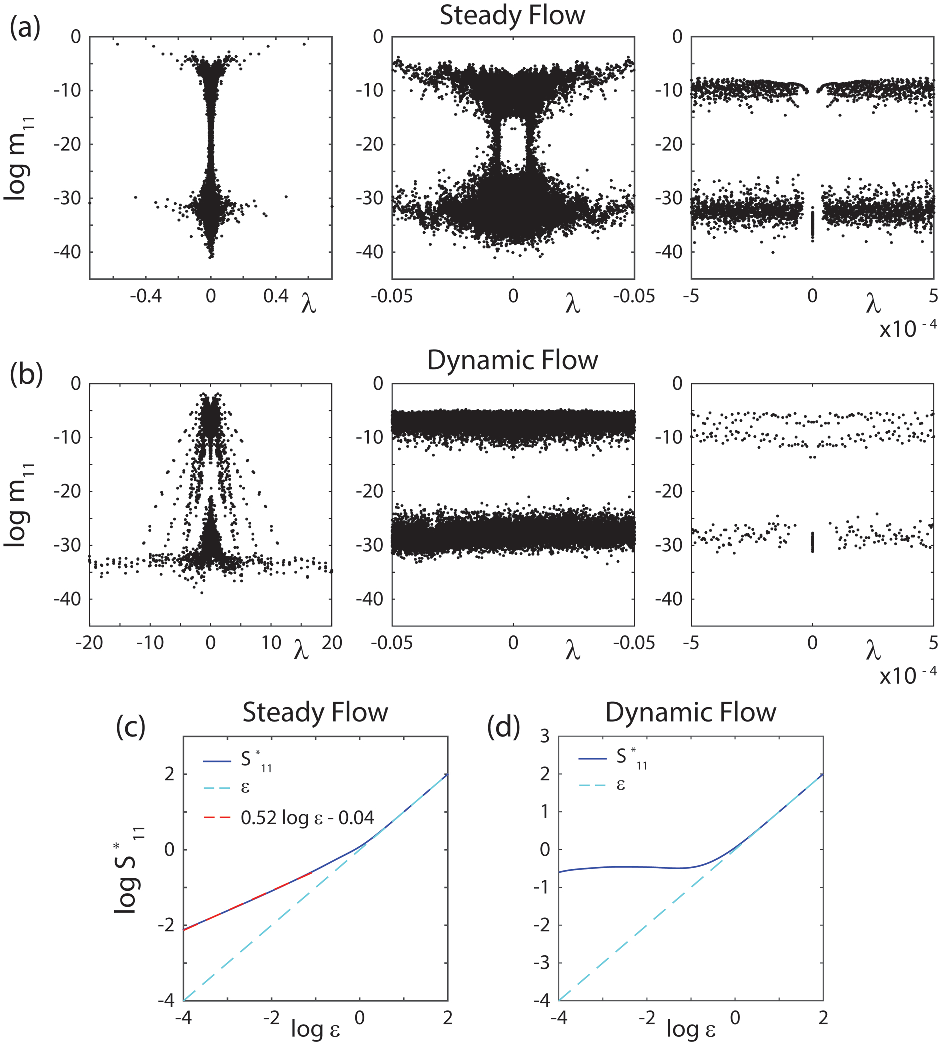
\includegraphics[scale=0.75]{Figure1_Spectral_Measures_Effective_Diffusivities}} 
\caption{%
  Computations of spectral measures and effective diffusivities for
  steady and dynamic flows. The spectral measure $\mu_{11}$ associated
  with the flow in~\eqref{eq:tdcell} are displayed for (a) the steady
  setting and (b) the dynamic setting with the associated effective
  diffusivity $\Sm^*_{11}$ displayed in (c) and (d), respectively. In
  the steady case (a), the 
  limit point of the measure near $\lambda=0$ has small measure mass with
  $m_{11}\lesssim10^{-30}$, leading to the asymptotic behavior
  $\Sm^*_{11}\sim\varepsilon^{1/2}$ for $\varepsilon\ll1$, displayed in (c). In the dynamic case
  (b), the significant measure mass $m_{11}\gtrsim10^{-10}$
  near $\lambda=0$ leads to the asymptotic behavior
  $\Sm^*_{11}\sim1$ for $\varepsilon\ll1$, displayed in (d).
        }
\label{fig:Fig1_Spect_Meas_Eff_Diffus}
\end{figure}
%


In summary, our numerical method is the following. Create the matrices
$\Bm$ and $\Cm$ according to equation~\eqref{eq:Fourier_Coef_System}
or~\eqref{eq:Fourier_Coef_System_Steady} and the corresponding
bijective mapping in~\eqref{eq:Bijections}. Remove the rows
and columns of the matrices $\Bm$ and $\Cm$ corresponding to
$\Cm_{ii}=0$. Compute the eigenvalues $\lambda_l$ and eigenvectors $\vecv_l$ of
the symmetric matrix $\Cm^{-1/2}\Bm\Cm^{-1/2}$. The computed Fourier
coefficients of the eigenfunction $\varphi_l$ are given by
$\veca_l=\Cm^{-1/2}\vecv_l$. The eigenvalues associated with the
discrete component of the spectral measure displayed in
equation~\eqref{eq:Stieltjes-Radon_Rep} are given by $\lambda_l$, while the
spectral measure weights $\langle g_1,\varphi_l\rangle_{1,2}$ and $\langle g_2,\varphi_l\rangle_{1,2}$
in~\eqref{eq:Stieltjes-Radon_Rep} are determined by the vector
$\veca_l$ via equation~\eqref{eq:Inner_Products_2D}
or~\eqref{eq:Inner_Products_2D_Steady}.     



In our computations, we used for the steady case $M=150$, yielding
matrices of size $(2M+1)^2-1=90,600$, while in the dynamic case we used
$M=20$, yielding matrices of size $(2M+1)^3-(2M+1)=68,880$. The
eigenvalues and eigenvectors of the symmetric matrix
$\Cm^{-1/2}\Bm\Cm^{-1/2}$ were computed using the Matlab function
\emph{eig()}. The stability of the computations are measured in terms
of the condition numbers $\mathcal{K}_l$ of the eigenvalues $\lambda_l$,
which are the reciprocals of the cosines of the angles between the
left and right eigenvectors. Eigenvalue condition numbers close to 1
indicate a stable computation. Our eigenvalue computations are
extremely stable with $\max_l|1-\mathcal{K}_l|\sim10^{-14}$, which were
computed using the Matlab function \emph{condeig()}.



Displayed in \figref{fig:Fig1_Spect_Meas_Eff_Diffus} are our
computations of the discrete component of the spectral measure
$\d\mu_{11}(\lambda)=\sum_lm_{11}(l)\delta_{\lambda_l}(\d\lambda)$ associated with the fluid
velocity field $\vecu$ displayed in equation~\eqref{eq:tdcell}, for (a)
the steady $(\theta=0)$ and (b) the dynamic $(\theta=1)$ settings. Here, the
spectral weights $m_{11}(l)=|\langle g_1,\varphi_l\rangle_{1,2}|^2$ are determined by
equations~\eqref{eq:Inner_Products_2D_Steady}
and~\eqref{eq:Inner_Products_2D}, respectively.  Consistent with the
symmetries of the flows~\cite{Biferale:PF:2725}, we have
$\mu_{11}=\mu_{22}$, while $\Real\mu_{12}=0$ and $\Imag\mu_{12}=0$, up to
numerical accuracy and finite size effects.




For the 2D steady cell
flow in~\eqref{eq:tdcell} with $\theta=0$, it is
known~\cite{Fannjiang:1994:SIAM_JAM:333,Novikov:2005:CPAM:867} that
$\Sm^*_{11}\sim\varepsilon^{1/2}$ for $\varepsilon\ll1$. Our computation of $\Sm^*_{11}$
displayed in \figref{fig:Fig1_Spect_Meas_Eff_Diffus}(c) is in
excellent agreement with this result, with a computed critical
exponent of $\approx0.52$ having an error of only $4\%$ relative to its true
value $0.5$. Reducing $M$ from 150 to 100 changes the value of the
critical exponent by less than $0.0015$, indicating that the value of
$M=150$ is sufficiently large. In this steady setting, the underlying
operator $(-\Delta)^{-1}[\vecu_1\cdot\bnabla]$ is
compact~\cite{Bhattacharya:AAP:1999:951} and therefore has 
bounded, discrete spectrum away from the spectral origin, with a limit
point at $\lambda=0$~\cite{Stakgold:BVP:2000}. The limit point behavior of  
the measure $\mu_{11}$ can be seen in the rightmost panel of
\figref{fig:Fig1_Spect_Meas_Eff_Diffus}(a). The decay of $\Sm^*_{11}$
for vanishing $\varepsilon$ is due to the magnitude of the measure masses
$m_{11}(l)\lesssim10^{-30}$ for $|\lambda_l|\ll1$, with a significant \emph{spectral
  gap} near the limit point. The rigorous
result~\cite{Fannjiang:1994:SIAM_JAM:333,Novikov:2005:CPAM:867} $\Sm^*_{11}\sim\varepsilon^{1/2}$ as
$\varepsilon\to0$ reveals that the spectrum of the operator
$(-\Delta)^{-1}[\vecu_1\cdot\bnabla]$ at $\lambda=0$ is either
continuous or it is discrete with zero mass,
otherwise $\Sm^*_{11}$ would diverge as $\varepsilon\to0$.  



In contrast, as shown in \figref{fig:Fig1_Spect_Meas_Eff_Diffus}(b),
the spectral measure $\mu_{11}$ associated with the time-dependent fluid
velocity field in~\eqref{eq:tdcell}, with $\theta=1$, has significant
values of $m_{11}(l)$ near the spectral origin, with
$m_{11}(l)\gtrsim10^{-10}$ more than \emph{20 orders} of magnitude greater
than  that of the steady flow. A limit point behavior in the measure
$\mu_{11}$ near $\lambda=0$ can be seen in the rightmost panel of
\figref{fig:Fig1_Spect_Meas_Eff_Diffus}(b).  It is interesting to note
that the support of the measure $supp\,\mu_{11}$ satisfies
$supp\,\mu_{11}\subset[-M,M]$ for all values of $M$ investigated. Due to
the significant mass of the measure near the spectral origin and its
uniform nature, as shown in the center panel of
\figref{fig:Fig1_Spect_Meas_Eff_Diffus}(b), the effective diffusivity
has an $O(1)$ behavior, $\Sm^*_{11}\sim1$ for $\varepsilon\ll1$, as shown in
\figref{fig:Fig1_Spect_Meas_Eff_Diffus}(d). This is consistent with 
numerical computations of $\Sm^*_{11}$ using alternate 
methods~\cite{Biferale:PF:2725}. This $O(1)$ behavior of $\Sm^*_{11}$
has been attributed to the Lagrangian chaotic behavior of the
flow~\cite{Biferale:PF:2725,ZCX_2015}. 



% %\newpage

% redefine the command that creates the equation no.
  \setcounter{equation}{1}  % reset equation counter
  \setcounter{section}{0}  % reset section counter
  \renewcommand{\theequation}{A-\arabic{equation}} 
\renewcommand{\thesection}{A-\arabic{section}}

\appendix
%
% \section{Appendix}\label{sec:Appendix}
% %

\section{Spectral theory of unbounded self-adjoint operators in
  Hilbert space} \label{app:Spectral_Theory}    
%
The theory of \emph{unbounded} operators in Hilbert
space was developed largely by John von Neumann and Marshall H. Stone. It
is considerably more technical and challenging than the theory of bounded
operators, as unbounded operators do not form an algebra, nor even a
linear space, because each one is defined on its own domain. In this
section, we review the spectral theory for such operators and, in
particular, the celebrated \emph{spectral theorem} for self-adjoint
operators~\cite{Reed-1980,Stone:64}.


An operator is not determined unless its domain is known. Let $\Phi_1$
and $\Phi_2$ be operators acting on a Hilbert space $\Hs$ with domains
$D(\Phi_1)$ and $D(\Phi_2)$, 
respectively, $D(\Phi_i)\subset\Hs$, $i=1,2$. They are said to be
\emph{identical}, in symbols $\Phi_1\equiv\Phi_2$, if and only if $D(\Phi_1)=D(\Phi_2)$
and $\Phi_1 f=\Phi_2 f$ for every $f$ of their common domain. They are said
to be \emph{equal} in 
the set $\mathscr{S}$, in symbols $\Phi_1=\Phi_2$, if and only if
$\mathscr{S}\subseteq D(\Phi_1)\cap D(\Phi_2)$ and $\Phi_1 f=\Phi_2 f$ for every
$f\in\mathscr{S}$. The operator $\Phi_2$ is said to be an \emph{extension}
(\emph{proper extension}) of the operator $\Phi_1$ if $D(\Phi_1)\subseteq D(\Phi_2)$
($D(\Phi_1)\subset D(\Phi_2)$) and the operators $\Phi_2$ and $\Phi_1$ are equal in
$D(\Phi_1)$~\cite{Stone:64}.   


Consider the sesquilinear inner-product $\langle\cdot,\cdot\rangle$ associated with $\Hs$
satisfying $\langle a\psi,b\varphi\rangle=a\,\overline{b}\,\langle\psi,\varphi\rangle$ and
$\langle\psi,\varphi\rangle=\overline{\langle\varphi,\psi\rangle}$ for all $\psi,\varphi\in\Hs$ and $a,b\in\mathbb{C}$, where
$\overline{z}$ denotes complex conjugation of $z\in\mathbb{C}$.
The $\Hs$--inner-product induces a norm $\|\cdot\|$ defined by
$\|\psi\|=\langle\psi,\psi\rangle^{1/2}$. A linear operator $\Phi$ is said to be \emph{closed}
if for every pair of sequences $\{f_n\}$ and $\{\Phi f_n\}$ (with $f_n\in D(\Phi)$)
that converge in the norm $\|\cdot\|$ to the limits $f$ and $h$, then 
$f\in D(\Phi)$ and $\Phi f=h$~\cite{Stone:64}. The (Hilbert space) 
adjoint $\Phi^*$ of $\Phi$ is   
defined by $\langle\Phi\psi,\varphi\rangle=\langle\psi,\Phi^*\varphi\rangle$ for every $\psi\in D(\Phi)$ and $\varphi\in D(\Phi^*)$. The
adjoint $\Phi^*$ of $\Phi$ is uniquely determined when the domain $D(\Phi)$
\emph{determines} $\Hs$, i.e., the smallest closed linear manifold
containing $D(\Phi)$ is the Hilbert space $\Hs$~\cite{Stone:64}. In this
case, $D(\Phi)\subseteq D(\Phi^*)$ and $\Phi^*$ is a closed linear
operator~\cite{Stone:64}. The operator $\Phi$ is said to be
\emph{symmetric} if $\Phi=\Phi^*$. The operator $\Phi$ is said to be
\emph{self-adjoint} if $\Phi\equiv\Phi^*$. A symmetric operator is said to be
\emph{maximal} if it has no proper symmetric extension. A self-adjoint
operator is a maximal symmetric operator~\cite{Stone:64}. 



The operator $\Phi$ is said to be \emph{bounded} (in operator norm) if
$\|\Phi\|=\sup_{\{\psi\in\Hs   \,:\, \|\psi\|=1\}}\|\Phi\psi\|<\infty$. A bounded linear symmetric
operator is self-adjoint if and only if its domain is
$\Hs$~\cite{Stone:64}. Conversely, the Hellinger--Toeplitz theorem
states that, if the operator $\Phi$ satisfies $\langle\Phi\psi,\varphi\rangle=\langle\psi,\Phi\varphi\rangle$ for \emph{every}
$\psi,\varphi\in\Hs$, then $\Phi$ is bounded on
$\Hs$~\cite{Reed-1980,Stone:64}. This indicates that, if $\Phi$ is an
\emph{unbounded} symmetric operator on $\Hs$, then it is self-adjoint
only on a \emph{proper subset} of $\Hs$ that is dense in $\Hs$. 



The spectrum $\Sigma$ of a self-adjoint operator $\Phi$ on a Hilbert space
$\Hs$ is real-valued~\cite{Reed-1980,Stone:64}. If $\Phi$ is also bounded,
then its spectral radius equal to its operator norm
$\|\Phi\|$~\cite{Reed-1980}, i.e., 
%
\begin{align}\label{eq:Spectral_Radius_Phi}
  \Sigma\subseteq[-\|\Phi\|,\|\Phi\|\,].
\end{align}
%
If $\Phi$ is instead unbounded, its spectrum $\Sigma$ can be an unbounded subset of,
or can even coincide with the set of real numbers
$\mathbb{R}$~\cite{Stone:64}.




We now summarize the spectral theorem for self-adjoint
operators (see Theorems 5.9 and  6.1 in~\cite{Stone:64}). Let
$\Phi$ be a fixed self-adjoint operator with spectrum $\Sigma\subseteq\mathbb{R}$ and 
domain $D(\Phi)$ that is dense in $\Hs$. If $\Phi$ is bounded
then we simply take $D(\Phi)\equiv\Hs$. The spectral theorem states that 
there is a one-to-one correspondence between the self-adjoint
operator $\Phi$ and a family of self-adjoint projection operators
$\{Q(\lambda)\}_{\lambda\in\Sigma}$ --- the resolution of the identity --- that
satisfies~\cite{Stone:64} 
%$\lim_{\lambda\to\,\inf{\Sigma}}Q(\lambda)=0$ and $\lim_{\lambda\to\,\sup{\Sigma}}Q(\lambda)=I$~\cite{Stone:64}
%
\begin{align}\label{eq:Res_Identity_limits}
  \lim_{\lambda\to\,\inf{\Sigma}}Q(\lambda)=0, \quad
  \lim_{\lambda\to\,\sup{\Sigma}}Q(\lambda)=I,
\end{align}
%
where $0$ and $I$ denote the null and identity operators on $\Hs$,
respectively. Furthermore, the \emph{complex-valued} function of the
spectral variable $\lambda$ defined by $\mu_{\psi\varphi}(\lambda)=\langle Q(\lambda)\psi,\varphi\,\rangle$ has real,
$\Real\mu_{\psi\varphi}(\lambda)$, and imaginary, $\Imag\mu_{\psi\varphi}(\lambda)$, parts that are
strictly increasing for $\lambda\in\Sigma$ and of bounded variation for all $\psi,\varphi\in
D(\Phi)$~\cite{Stone:64}, where
%
\begin{align}\label{eq:Fns_Bounded_Var}
  \Real\mu_{\psi\varphi}(\lambda)
         &=\frac{1}{2}\left(\mu_{\psi\varphi}(\lambda)+\overline{\mu}_{\psi\varphi}(\lambda)\right),
  \\
  \Imag\mu_{\psi\varphi}(\lambda)
         &=\frac{1}{2\,\imath}\left(\mu_{\psi\varphi}(\lambda)-\overline{\mu}_{\psi\varphi}(\lambda)\right),
  \notag
\end{align}
%
$\imath=\sqrt{-1}$, and $\lambda\in\Sigma$.





By the sesquilinearity of the inner-product and the fact that the
projection operator $Q(\lambda)$ is self-adjoint, the function $\mu_{\psi\varphi}(\lambda)$
satisfies $\mu_{\varphi\psi}(\lambda)=\overline{\mu}_{\psi\varphi}(\lambda)$. Moreover, the function
$\mu_{\psi\psi}(\lambda)$ is real-valued and positive, $\mu_{\psi\psi}(\lambda)=\langle Q(\lambda)\psi,\psi\rangle=\langle
Q(\lambda)\psi,Q(\lambda)\psi\rangle=\|Q(\lambda)\psi\,\|^2\geq0$, hence $\Real\mu_{\psi\psi}(\lambda)=\mu_{\psi\psi}(\lambda)$ and
$\Imag\mu_{\psi\psi}(\lambda)=0$. With each of these strictly increasing functions
of bounded variation, we associate Stieltjes
measures~\cite{Stieltjes:1995,Stone:64,Folland:99:RealAnalysis}  
%
\begin{align}\label{eq:Bounded_Variation}
  &\d\mu_{\psi\varphi}(\lambda)=\d\langle Q(\lambda)\psi,\varphi\rangle, \qquad
  \d\Real\mu_{\psi\varphi}(\lambda)=\d\Real\langle Q(\lambda)\psi,\varphi\rangle,\\  
  &\d\mu_{\psi\psi}(\lambda)=\d\|Q(\lambda)\psi\,\|^2, \qquad
  \hspace{0.2em}
  \d\Imag\mu_{\psi\varphi}(\lambda)=\d\Imag\langle Q(\lambda)\psi,\varphi\rangle,
  \notag
\end{align}
%
which we will denote by $\mu_{\psi\psi}$, $\mu_{\psi\varphi}$, $\Real\mu_{\psi\varphi}$, and
$\Imag\mu_{\psi\varphi}$. We stress that $\mu_{\psi\psi}$ is a positive measure, $\mu_{\psi\varphi}$
is a complex measure, while $\Real\mu_{\psi\varphi}$ and $\Imag\mu_{\psi\varphi}$ are signed
measures~\cite{Stieltjes:1995,Stone:64}.  



The spectral theorem also provides an operational calculus in Hilbert
space which yields powerful integral representations involving the
Stieltjes measures displayed in
equation~\eqref{eq:Bounded_Variation}. A summary of the relevant
details are as   
follows. Let $F(\lambda)$ and $G(\lambda)$ be arbitrary complex-valued functions
and denote by $\Ds(F)$ the set of all $\psi\in D(\Phi)$ such that
$F\in L^2(\mu_{\psi\psi})$, i.e., $F$ is square integrable on the set
$\Sigma$ with respect to the \emph{positive} measure $\mu_{\psi\psi}$, and similarly define
$\Ds(G)$. Then $\Ds(F)$ and $\Ds(G)$ are linear manifolds and there
exist linear operators denoted by $F(\Phi)$ and $G(\Phi)$ with domains
$\Ds(F)$ and $\Ds(G)$, respectively, which are defined in terms of the
following Radon--Stieltjes integrals~\cite{Stone:64}  
%
\begin{align}\label{eq:Spectral_Theorem}
  \langle F(\Phi)\psi,\varphi\rangle&=\int_{-\infty}^\infty F(\lambda)\,\d\mu_{\psi\varphi}(\lambda), \qquad
  \hspace{1em}
  \forall \, \psi\in\mathscr{D}(F), \ \varphi\in D(\Phi),  
  \\
  \langle F(\Phi)\psi,G(\Phi)\varphi\rangle&=\int_{-\infty}^\infty F(\lambda)\overline{G}(\lambda)\,\d\mu_{\psi\varphi}(\lambda),
  \quad
  \forall \, \psi\in\mathscr{D}(F), \ \varphi\in\mathscr{D}(G),
  \notag
\end{align}
%
where the integration in~\eqref{eq:Spectral_Theorem} is over the
spectrum $\Sigma$ of $\Phi$~\cite{Reed-1980,Stone:64}.



The mass $\mu^0_{\psi\varphi}=\int_{-\infty}^\infty\d\mu_{\psi\varphi}(\lambda)$ of the
Stieltjes measure $\mu_{\psi\varphi}$ satisfies~\cite{Stone:64}
$\mu^0_{\psi\varphi}=\lim_{\lambda\to\sup\Sigma}\mu_{\psi\varphi}(\lambda)-\lim_{\lambda\to\inf\Sigma}\mu_{\psi\varphi}(\lambda)$. Consequently,
equation~\eqref{eq:Res_Identity_limits} and the Cauchy-Schwartz
inequality yield
% 
\begin{align}\label{eq:Mass_General}
  \mu^0_{\psi\varphi}=\int_{-\infty}^\infty\d\langle Q(\lambda)\psi,\varphi\,\rangle=\langle\psi,\varphi\rangle,
  \qquad
  |\mu^0_{\psi\varphi}|\leq\|\psi\|\,\|\varphi\|<\infty.
\end{align}
%
Equation~\eqref{eq:Mass_General} demonstrates that the measures
in~\eqref{eq:Bounded_Variation} are \emph{finite measures}, i.e., they
have bounded mass~\cite{Stone:64}.




Equation~\eqref{eq:Spectral_Theorem} can be generalized, holding with
suitable notational changes, for \emph{maximal normal
  operators}~\cite{Stone:64}. Such a normal operator $\Nb$ with domain
$D(\Nb)$ dense in $\Hs$ commutes with its adjoint $\Nb^*$, i.e., 
$\Nb\Nb^*=\Nb^*\Nb$, and can be decomposed as $\Nb=\Phi_1+\imath\Phi_2$, where
$\Phi_1$ and $\Phi_2$ are self-adjoint and commute. The spectrum of the
normal operator $\Nb$ is 
a (possibly unbounded) subset of $\mathbb{C}$~\cite{Stone:64}. A
special case of a normal operator is a \emph{skew-adjoint} operator
satisfying $\Nb^*=-\Nb$. It can be decomposed as $\Nb=\imath\Phi_2$ and since
$\Phi_2$ is self-adjoint having purely real spectrum, the skew-adjoint
operator $\Nb=\imath\Phi_2$ has purely imaginary
spectrum~\cite{Stone:64}. Consequently, given such a maximal
skew-adjoint operator, one can focus attention on the self-adjoint
operator $\Phi_2=-\imath\Nb$ without having to resort to the more notationally
complicated spectral theory of normal operators.





The signed measures $\Real\mu_{\psi\varphi}$ and $\Imag\mu_{\psi\varphi}$ displayed in
equation~\eqref{eq:Bounded_Variation} arise naturally when considering
a maximal skew-adjoint operator $\Nb=\imath\Phi$, where $\Phi$ is
self-adjoint. This can be illustrated by considering some special
cases. Consider the functional $\langle F(\Nb)\psi,G(\Nb)\varphi\rangle$ involving
\emph{real-valued} Hilbert space members $F(\Nb)\psi$ and $G(\Nb)\varphi$, so
that $\langle F(\Nb)\psi,G(\Nb)\varphi\rangle=\langle G(\Nb)\varphi,F(\Nb)\psi\rangle\in\mathbb{R}$ and, in
particular, 
%$\langle F(\Nb)\psi,G(\Nb)\varphi\rangle=(\langle F(\Nb)\psi,G(\Nb)\varphi\rangle+\langle G(\Nb)\varphi,F(\Nb)\psi\rangle)/2$.
%
\begin{align}\label{eq:Real_Val_Functional}
  \langle F(\Nb)\psi,G(\Nb)\varphi\rangle=\frac{1}{2}(\langle F(\Nb)\psi,G(\Nb)\varphi\rangle+\langle G(\Nb)\varphi,F(\Nb)\psi\rangle).
\end{align}
%
Now consider the special cases $F(\Nb)=G(\Nb)$ and $F(\Nb)=\Nb G(\Nb)$,
i.e., $F(\imath\lambda)=G(\imath\lambda)$ and $F(\imath\lambda)=\imath\lambda G(\imath\lambda)$ in
equation~\eqref{eq:Spectral_Theorem}, respectively. It follows 
from equations~\eqref{eq:Spectral_Theorem}
and~\eqref{eq:Real_Val_Functional}, the identities
$\Real z=(z+\overline{z})/2$ and $\Imag z=(z-\overline{z})/(2\imath)$, and
the linearity properties~\cite{Stone:64} of Stieltjes-Radon integrals
with respect to the functions $\mu_{\psi\varphi}(\lambda)$ and $\overline{\mu}_{\psi\varphi}(\lambda)$ that
%
\begin{align}\label{eq:Real_Imag_mu_Reps}
  \langle G(\Nb)\psi,G(\Nb)\varphi\rangle&=\int_{-\infty}^\infty|G(\imath\lambda)|^2\,\d\Real\mu_{\psi\varphi}(\lambda),
  \\
   \langle\Nb G(\Nb)\psi,G(\Nb)\varphi\rangle&=-\int_{-\infty}^\infty\lambda\,|G(\imath\lambda)|^2\,\d\Imag\mu_{\psi\varphi}(\lambda).
   \notag
\end{align}
%




An important property of a self-adjoint operator $\Phi$ which will be
used later is that its domain $D(\Phi)$ comprises those and only those
elements $\psi\in\Hs$ such that the Stieltjes integral
$\int_{-\infty}^\infty\lambda^2\,\d\mu_{\psi\psi}(\lambda)$ is convergent. When $\psi\in D(\Phi)$ the element
$\Phi\psi$ is determined by the relations~\cite{Stone:64}      
%
\begin{align}\label{eq:X_Q_Correspondence}
  \langle\Phi\psi,\varphi\rangle=\int_{-\infty}^\infty\lambda\,\d\mu_{\psi\varphi}(\lambda), \qquad
  \|\Phi\psi\|^2=\int_{-\infty}^\infty\lambda^2\,\d\mu_{\psi\psi}(\lambda),
\end{align}
%
where $\varphi$ is an arbitrary element in $D(\Phi)$~\cite{Stone:64}. In fact,
this determines the one-to-one correspondence between the
self-adjoint operator $\Phi$ and its resolution of the identity
$Q(\lambda)$~\cite{Stone:64}. 





\section{Time derivative as a maximal normal
  operator}\label{app:Time_Derivative}
%
A key example of an unbounded operator is the time derivative
$\partial_t$ acting on the space $L^2(\Tc)$ of Lebesgue measurable functions
that are also square integrable on the interval $\Tc=[0,T]$, say. The
unboundedness of $\partial_t$ as an operator on $L^2(\Tc)$ can be 
understood by considering the orthonormal set of functions
$\{\varphi_n\}\subset L^2(\Tc)$ defined by     
%
\begin{align}\label{eq:Orthonormal}
  \varphi_n(t)=\beta\sin(n\pi t/T), \quad
  \beta=\sqrt{2/T},
  \qquad
  \langle\varphi_n,\varphi_m\rangle_2=\delta_{nm},
  %\quad
  %n,m\in\mathbb{N},
\end{align}
%
where $n,m\in\mathbb{N}$ and $\langle\cdot,\cdot\rangle_2$ denotes the sesquilinear
$L^2(\Tc)$--inner-product. It follows from $\partial_t\varphi_n=(n\pi\beta/T)\cos(n\pi t/T)$
and $\|\partial_t\varphi_n\|^2=(n\pi/T)^2$, that the norm of the members of the set
$\{\partial_t\varphi_n\}$ grows arbitrarily large as $n\to\infty$. This clearly demonstrates
the unboundedness of the operator $\partial_t$ with domain $L^2(\Tc)$.





When one also imposes periodic or Dirichlet boundary conditions,
simple integration by parts demonstrates that the operator $\partial_t$ is
\emph{skew-symmetric} on $L^2(\Tc)$ so that $-\imath\partial_t$ is symmetric with
respect to the sesquilinear inner-product $\langle\cdot,\cdot\rangle_2$. We now identify an
everywhere dense subset of $L^2(\Tc)$ on which $-\imath\partial_t$ is a bounded
linear self-adjoint operator~\cite{Reed-1980,Stone:64}. Consider the
class $\As_{\Tc}$ of all functions $\psi\in L^2(\Tc)$ such that $\psi(t)$ is
\emph{absolutely continuous}~\cite{Royden:1988:RA} on the interval
$\Tc$ and has a derivative $\psi^{\,\prime}(t)$ belonging to $L^2(\Tc)$,
i.e.,~\cite{Stone:64,Royden:1988:RA}     
%
\begin{align}\label{eq:AC_L2}
  \As_{\Tc}=
     \left\{
       \psi\in L^2(\Tc) \ \Big| \ \psi(t)=c+\int_0^tg(s)ds,
       \quad  g\in L^2(\Tc)
     \right\},
\end{align}
%
where the constant $c$ and function $g(s)$ are
arbitrary. Now, consider the set $\tilde{\As}_{\Tc}$ of all
functions $\psi\in\As_{\Tc}$ that satisfy the periodic boundary condition
$\psi(0)=\psi(T)$, i.e. functions $\psi$ satisfying the properties of 
equation~\eqref{eq:AC_L2} with $\int_0^Tg(s)ds=0$. In order to help
clarify the ideas that were discussed in~\appref{app:Spectral_Theory}
in terms of an abstract 
Hilbert space $\Hs$, we also consider the set $\hat{\As}_{\Tc}$ of all
functions $\psi\in\As_{\Tc}$ that satisfy the Dirichlet boundary condition
$\psi(0)=\psi(T)=0$, i.e. functions $\psi$ satisfying the properties of
equation~\eqref{eq:AC_L2} with $c=0$ and $\int_0^Tg(s)ds=0$. More
concisely,  
%
\begin{align}\label{eq:AC_BC}
  \tilde{\As}_{\Tc}&=\{\psi\in\As_{\Tc} \,|\, \psi(0)=\psi(T)\},
  \\
  \hat{\As}_{\Tc}&=\{\psi\in\As_{\Tc} \,|\, \psi(0)=\psi(T)=0\}.
  \notag
\end{align}
%
These function spaces satisfy
$\hat{\As}_{\Tc}\subset\tilde{\As}_{\Tc}\subset\As_{\Tc}$ and are each everywhere
dense in $L^2(\Tc)$~\cite{Stone:64}. Let the operators $B$,
$\tilde{B}$, and $\hat{B}$ be identified as $-\imath\partial_t$ with domains
$\As_{\Tc}$, $\tilde{\As}_{\Tc}$, and $\hat{\As}_{\Tc}$,
respectively. Then, $\hat{B}$ is a closed linear symmetric operator
with the adjoint $\hat{B}^*\equiv B$, and the operator $\tilde{B}$ is a
\emph{self-adjoint} extension of $\hat{B}$~\cite{Stone:64}. In
symbols, this means that $\tilde{B}=\tilde{B}^*$ on
$\tilde{\As}_{\Tc}$ and
$D(\tilde{B})=D(\tilde{B}^*)=\tilde{\As}_{\Tc}$,
i.e., $\tilde{B}\equiv\tilde{B}^*$ on $\tilde{\As}_{\Tc}$. This establishes
that the operator $-\imath\partial_t$ with domain $\tilde{\As}_{\Tc}$ is
self-adjoint, hence $\partial_t$ is a maximal skew-symmetric (normal)
operator on $\tilde{\As}_{\Tc}$. The operator $\imath\partial_t$ on
$\tilde{\As}_{\Tc}$ has a simple point spectrum, consisting of
eigenvalues $\lambda=2n\pi/T$, $n\in\mathbb{Z}$, with corresponding
eigenfunctions $\exp(\imath\,2n\pi t/T)$~\cite{Stone:64}.





\section{Hilbert spaces, resolvents, and integral representations of the effective diffusivity}
\label{app:Hilbert_Resolvent_Integral_Reps} 
%
In this section we formulate a spectral theory of effective
diffusivities for space-time periodic
flows. In~\appref{app:Scalar_Fields} we address an approach suggested
in~\cite{Pavliotis:PHD_Thesis}, while in~\appref{app:Curl_Free_Fields}
we address an approach suggested in~\cite{Avellaneda:PRE:3249}. In 
each case, we provide a rigorous mathematical framework which leads to
Stieltjes integral representations for both the symmetric $\Sm^*$ and
antisymmetric $\Am^*$ parts of the effective diffusivity tensor
$\Dm^*$ for space-time periodic
flows, involving a spectral measure of an \emph{unbounded}
self-adjoint operator. In~\appref{app:Isometric_Correspondence} we use
the one-to-one correspondence between a self-adjoint operator and its
resolution of the identity~\cite{Stone:64}, discussed in the paragraph
containing equation~\eqref{eq:X_Q_Correspondence}, to establish that
the two approaches are equivalent.  



\subsection{Scalar fields and the effective diffusivity}\label{app:Scalar_Fields}
%
In this section we provide an abstract Hilbert space formulation of
the effective parameter problem for advection enhanced diffusion by a
space-time periodic fluid velocity field $\vecu(t,\vecx)$. To fix
ideas, consider the following sets $\Tc=[0,T]$ and
$\Vc=\otimes_{j=1}^d[0,\ell]$ which  define the space-time period cell
$\Tc\times\Vc$ for $\vecu(t,\vecx)$. Now consider the Hilbert spaces
$L^2(\Tc)$ and $L^2(\Vc)$ of Lebesgue measurable functions over the
complex field $\mathbb{C}$ that are also square integrable on $\Tc$
and $\Vc$, respectively.  Define the associated Hilbert spaces
$\Hs_{\Tc}$ and $\Hs_{\Vc}$, 
%as well as their direct product $\Hs_{\Tc\Vc}=\Hs_{\Tc}\otimes\Hs_{\,\Vc}$ 
%$\Hs_{\Tc\Vc}$,
%
\begin{align}\label{eq:Hilbert_Spaces_scalar}
  %\Hs_{\Tc\Vc}=\Hs_{\Tc}\otimes\Hs_{\,\Vc}, \quad
  \Hs_{\Tc}&=\big\{\psi\in L^2(\Tc) \, | \, \psi(t)=\psi(t+T), \ \langle\psi\rangle_{\Tc}=0\big\},
  \\
  \Hs_{\Vc}&=\big\{\psi\in L^2(\Vc) \, | \, \psi(\vecx)=\psi(\vecx+\ell\vece_j), \ \langle\psi\rangle_{\Vc}=0\big\},
  \notag
\end{align}
%
for all $j=1,\ldots,d$, where the $\vece_j$ are standard basis
vectors. Here, $\langle\cdot\rangle_{\Tc}$ and $\langle\cdot\rangle_{\Vc}$ denote temporal average
over $\Tc$ and spatial average over $\Vc$, respectively. Denote by 
$\langle\cdot\rangle$ space-time averaging over $\Tc\times\Vc$. Now define the Hilbert space 
$\Hs_{\Tc\Vc}=\Hs_{\Tc}\otimes\Hs_{\Vc}$ with sesquilinear
inner-product $\langle\cdot,\cdot\rangle$ given by $\langle\psi,\varphi\rangle=\langle\psi\,\overline{\varphi}\rangle$, with
$\langle\varphi,\psi\rangle=\overline{\langle\psi,\varphi\rangle}$. The $\Hs_{\Tc\Vc}$--inner-product induces a
norm $\|\cdot\|$ given by  $\|\psi\|=\langle\psi,\psi\rangle^{1/2}$~\cite{Folland:99:RealAnalysis}. 



In equation~\eqref{eq:AC_BC} we defined the space $\tilde{\As}_{\Tc}$ of
absolutely continuous $\Tc$-periodic functions with time derivatives
belonging to $L^2(\Tc)$. In view of the definition of $\Hs_{\Tc}$
in~\eqref{eq:Hilbert_Spaces_scalar}, we now define
%
\begin{align}
  \tilde{\As}^{\,0}_{\Tc}=\tilde{\As}_{\Tc}\cap\Hs_{\Tc}
                  =\{\psi\in\tilde{\As}_{\Tc}\,|\,  \langle\psi\rangle_{\Tc}=0\},
\end{align}
%
%In \appref{app:Time_Derivative} discussed that $\tilde{\As}^{\,0}_{\Tc}$
which is \emph{not} a Hilbert space but is instead an everywhere dense
subset of the Hilbert space $\Hs_{\Tc}$~\cite{Stone:64}. To treat
spatial dependence, we define
the Sobolev space $\Hs^{1,2}_{\Vc}$ which is itself a Hilbert
space~\cite{Bhattacharya:AAP:1999:951,Folland:95:PDEs,McOwen:2003:PDE},             
% 
\begin{align}\label{eq:Sobolev}
  \Hs^{1,2}_{\Vc}=\big\{\psi\in \Hs_{\Vc} \; | \; \langle|\bnabla \psi|^2\rangle_{\Vc}<\infty\big\}.
\end{align}
%
More specifically, the Sobolev space $\Hs^{1,2}_{\Vc}$  is the
closure in the norm $\langle|\bnabla\psi|^2\rangle_{\Vc}$ of the space of all twice
continuously differentiable periodic functions in $\Hs_{\Vc}$, and all
the elements of $\Hs^{1,2}_{\Vc}$ are those elements of $\Hs_{\Vc}$ which
have square integrable gradients on the set
$\Vc$~\cite{Bhattacharya:AAP:1999:951}.





Finally, consider the Hilbert
space $\Hs$ and its everywhere dense subset $\Fs$ defined by
%
\begin{align}\label{eq:Function_Space_Scalar}
  \Hs=\Hs_{\Tc}\otimes\Hs^{1,2}_{\Vc}, \qquad
  \Fs=\tilde{\As}^{\,0}_{\Tc}\otimes\Hs^{1,2}_{\Vc}.
  %\Hs=\big\{\psi\in\Hs_{\Tc}\otimes\Hs^{1,2}_{\Vc} \; | \; \langle \psi\rangle=0\big\}, \qquad
  %\Fs=\big\{\psi\in\tilde{\As}^{\,0}_{\Tc}\otimes\Hs^{1,2}_{\Vc} \; | \; \langle \psi\rangle=0\big\}.
  %\langle \psi,g\rangle_{1,2}=\left\langle\overline{\bnabla \psi}\cdot\bnabla g\right\rangle,
\end{align}
%
We stress that $\tilde{\As}^{\,0}_{\Tc}$ and $\Fs$ are \emph{not} a
complete Hilbert spaces. Instead, they are everywhere dense subsets of
the complete Hilbert spaces $\Hs_{\Tc}$ and $\Hs$, respectively.
Recalling that $\vecpsi\cdot\vecvarphi=\vecpsi^T\overline{\vecvarphi}$,
the sesquilinear  
$\Hs$--inner-product is given by $\langle\psi,\varphi\rangle_{1,2}=\left\langle\bnabla \psi\cdot\bnabla \varphi \right\rangle$ with associated norm
$\|\cdot\|_{1,2}$ given by $\|\psi\|_{1,2}= \langle|\bnabla \psi|^2\rangle^{1/2}$. Since $\langle|\partial_t\psi|^2\rangle_{\Tc}<\infty$ for all $\psi\in\tilde{\As}_{\Tc}$
  and $\langle|\bnabla \psi|^2\rangle_{\Vc}<\infty$ for all $\psi\in\Hs^{1,2}_{\Vc}$, it follows
  that $\|\partial_t\psi\|_{1,2}^2=\langle|\bnabla \partial_t\psi|^2\rangle<\infty$ and $\|\psi\|_{1,2}<\infty$ for all
  $\psi\in\Fs$. In the case of a
time-independent fluid velocity field $\vecu(\vecx)$ we set
$\Hs\equiv\Fs\equiv\Hs^{1,2}_{\Vc}$.  





We now use properties of the Hilbert space $\Hs$ to obtain
functional formulas for the symmetric $\Sm^*$ and antisymmetric
$\Am^*$ parts of the effective diffusivity tensor $\Dm^*$ defined in
equations~\eqref{eq:Djk} and~\eqref{eq:Symm_Anti-Symm}, involving the
solution $\chi_j$ of the cell problem in
equation~\eqref{eq:Periodic_Cell_Prob} and a maximal skew-symmetric
operator $A$ on $\Fs$. We then derive from the cell 
problem a resolvent formula for $\chi_j$ involving the operator
$A$. The spectral theorem discussed in~\appref{app:Spectral_Theory}
then yields Stieltjes integral representations for
$\Sm^*$ and $\Am^*$, which will be established in
\thmref{thm:Integral_Reps} below. 


Applying the linear operator $(-\Delta)^{-1}$ to both sides of the cell
problem in equation~\eqref{eq:Periodic_Cell_Prob} yields
%$(-\Delta)^{-1}u_j=[\varepsilon+(-\Delta)^{-1}(\partial_t-\vecu\cdot\bnabla)]\chi_j$.
%
\begin{align}\label{eq:Pre_Resolvent_Scalar}
  (-\Delta)^{-1}u_j=(\varepsilon+A)\chi_j,
  \qquad
  A=(-\Delta)^{-1}(\partial_t-\vecu \cdot\bnabla).
\end{align}
%
%where we have defined $A=(-\Delta)^{-1}(\partial_t-\vecu \cdot\bnabla)$.
We will discuss the key properties of the operators $(-\Delta)^{-1}$ and
$A$ in more detail below.  Now write the functional $\langle u_j\chi_k\rangle$ in 
equation~\eqref{eq:Djk} as~\cite{Pavliotis:PHD_Thesis}       
%
\begin{align}\label{eq:uj_chik}
  \langle u_j\chi_k\rangle=\langle[\Delta\Delta^{-1}u_j]\,\chi_k\rangle
       =-\langle\bnabla \Delta^{-1}u_j\cdot\bnabla \chi_k\rangle
       =\langle(-\Delta)^{-1}u_j,\chi_k\rangle_{1,2}.
\end{align}
%
This calculation will be rigorously justified in the proof of
\thmref{thm:Integral_Reps} below. Substituting the  
formula for $(-\Delta)^{-1}u_j$ in~\eqref{eq:Pre_Resolvent_Scalar} into
equation~\eqref{eq:uj_chik} yields
equation~\eqref{eq:Eff_Diffusivity_Sobolev}, with appropriate
notational changes, which provides functional
formulas for the components
$\Sm^*_{jk}$ and $\Am^*_{jk}$, $j,k=1,\ldots,d$, of $\Sm^*$ and $\Am^*$.
Equation~\eqref{eq:Pre_Resolvent_Scalar}   
leads to the resolvent formula displayed in
equation~\eqref{eq:Resolvent_Rep_Scalar}. 
From equations~\eqref{eq:Eff_Diffusivity_Sobolev}
and~\eqref{eq:Resolvent_Rep_Scalar} we have the functional formulas 
for $\Sm^*_{jk}$ and $\Am^*_{jk}$ displayed in
equation~\eqref{eq:Eff_Diff_Resolvent_Sobolev} involving the resolvent
of the operator $A$. The following theorem establishes the 
Stieltjes integral representations  in~\eqref{eq:Integral_Rep_kappa*}
for these functional formulas of $\Sm^*_{jk}$ and $\Am^*_{jk}$. 



%
\begin{theorem}\label{thm:Integral_Reps}
  The operator $A=(-\Delta)^{-1}(\partial_t-\vecu\cdot\bnabla)$ defined in
  equation~\eqref{eq:Pre_Resolvent_Scalar} is a maximal 
  (skew-symmetric) normal operator on the function space $\Fs$ defined
  in equation~\eqref{eq:Function_Space_Scalar}, hence $M=-\imath A$ is 
  self-adjoint on $\Fs$. Let $Q(\lambda)$ be the resolution of the
  identity in one-to-one correspondence with $M$. Define the complex
  valued   function $\mu_{jk}(\lambda)=\langle Q(\lambda)g_j,g_k\rangle_{1,2}$, $j,k=1,\ldots,d$, where
  $g_j=(-\Delta)^{-1}u_j$ is defined in~\eqref{eq:Resolvent_Rep_Scalar} and 
  $\langle\cdot,\cdot\rangle_{1,2}$ is the $\Hs$--inner-product. Consider the positive measure
  $\mu_{kk}$ and the signed measures $\Real\mu_{jk}$ and $\Imag\mu_{jk}$
  associated with $\mu_{jk}(\lambda)$, introduced in~\eqref{eq:Fns_Bounded_Var}.  Then, for
  $u_j\in\tilde{\As}^{\,0}_{\Tc}\otimes\Hs_{\Vc}$ and $\chi_j\in\Fs$
  %$u_j$ and $\chi_j$ satisfying equation~\eqref{eq:Min_Cond_uj_chij} 
  and all $0<\varepsilon<\infty$,
  the functional formulas for $\Sm^*_{jk}$ and $\Am^*_{jk}$ 
  in~\eqref{eq:Eff_Diff_Resolvent_Sobolev} have the 
  Radon--Stieltjes integral representations displayed in
  equation~\eqref{eq:Integral_Rep_kappa*}.   
% 
\end{theorem}
%


Before proving \thmref{thm:Integral_Reps}, we discuss key
properties of the linear operator $(-\Delta)^{-1}$. The Laplacian $\Delta$ maps
constants to the null element $0$ and periodic 
functions to periodic functions. In~\eqref{eq:Periodic_Cell_Prob} the 
operator $\Delta$ is acting on a periodic function. Hence, in the present
context, the domain of the operator $(-\Delta)^{-1}$ is mean-zero periodic
functions. The operator is $(-\Delta)^{-1}$ based on convolution
with respect to the Green's function for the Laplacian, i.e.,
$(-\Delta)^{-1}f(\vecx)=\int_{\Vc}G(\vecx-\vecy)\,f(\vecy)\d\vecy$. The
Green's function $G$ is determined by the sum of a
fundamental solution for the Laplacian and a harmonic function with,
in the present contex, periodic boundary conditions on
$\Vc$~\cite{Folland:95:PDEs,McOwen:2003:PDE,Stakgold:BVP:2000}. It is
positive, $G>0,$ symmetric, $G(\vecx-\vecy)=G(\vecy-\vecx)$, and
integrable~\cite{Folland:95:PDEs,Stakgold:BVP:2000} (see
Proposition 0.5 in~\cite{Folland:95:PDEs}) 
%
\begin{align}
 \sup_{\vecx\in\Vc} \int_{\Vc}G(\vecx-\vecy)\d\vecy\leq C<\infty.
\end{align}
%
Consequently, by Young's inequality, $(-\Delta)^{-1}$ is a bounded operator
on $L^p(\Vc)$ for all $1\leq
p\leq\infty$~\cite{Folland:95:PDEs,Folland:99:RealAnalysis}. More
specifically, if $\psi\in L^p(\Vc)$ 
then $(-\Delta)^{-1}\psi\in L^p(\Vc)$ and   
%
\begin{align}\label{eq:Young_Ineq}
  \|(-\Delta)^{-1}\psi\|_p\leq C\|\psi\|_p,
  \quad
  1\leq p\leq\infty,
\end{align}
%
where $\|\cdot\|_p$ denotes the $L^p(\Vc)$-norm. 



 Integration by parts, the Cauchy-Schwartz inequality,
$|\langle f,g\rangle|\leq\|f\|_2\,\|g\|_2$, and Young's inequality for $p=2$ imply for
$\psi\in\Hs_{\Vc}$ that
%
\begin{align}
  \langle|\bnabla(-\Delta)^{-1}\psi|^2\rangle_{\Vc}&=|\langle\bnabla(-\Delta)^{-1}\psi\bcdot\bnabla(-\Delta)^{-1}\psi\rangle_{\Vc}|
              \\
              &=|\langle(-\Delta)^{-1}\psi,\psi\rangle_{\Vc}|
              \notag\\
              &\leq C\|\psi\|_{\Vc}^2<\infty.
              \notag
\end{align}
%
Consequently, the operator $(-\Delta)^{-1}$ maps $\Hs_{\Vc}$ to
$\Hs^{1,2}_{\Vc}\cup\mathbb{C}$ (since $\Delta^{-1}\psi$ is not necessarily
mean-zero for $\psi\in\Hs_{\Vc}$). However, recalling that
$\Fs=\tilde{\As}^{\,0}_{\Tc}\otimes\Hs^{1,2}_{\Vc}$, since $\psi\in\Fs$ implies
that $\psi$ is mean-zero in both space and time, Fubini's
theorem~\cite{Folland:99:RealAnalysis} yields 
% $(-\Delta)^{-1}:L^2(\Vc)\to\Hs^{1,2}_{\Vc}$.
%
\begin{align}\label{eq:L2_to_H1}
  (-\Delta)^{-1}:\tilde{\As}^{\,0}_{\Tc}\otimes\Hs_{\Vc}\to\Fs.
\end{align}
%
It is important to note that in
equation~\eqref{eq:Eff_Diff_Resolvent_Sobolev}, other 
than the implicit appearance of $\vecu$ in the operator $A$, the
components $u_j$, $j=1,\ldots,d$, of the fluid velocity field enter into
the functional representations of $\Sm^*_{jk}$ and $\Am^*_{jk}$ only
through the auxillary function $g_j=(-\Delta)^{-1}u_j$. In light of this
and equation~\eqref{eq:L2_to_H1}
%, and the requirement of the spectral theorem
%in~\eqref{eq:Spectral_Theorem} that $g_j\in\Fs$, as we discuss in detail
%in the proof of \thmref{thm:Integral_Reps},
we will 
henceforth assume that    
%$(-\Delta)^{-1}u_j,\chi_j\in\Fs$ 
%for all $j=1,\ldots,d$,
%
\begin{align} \label{eq:Min_Cond_uj_chij}
 %u_j,\chi_j\in\Fs.
 u_j\in\tilde{\As}^{\,0}_{\Tc}\otimes\Hs_{\Vc},
 %\qquad
 %\chi_j\in\tilde{\As}^{\,0}_{\Tc}\otimes\Hs^{1,2}_{\Vc},
 %\chi_j\in\Fs
 %\qquad
 j=1,\ldots,d,
\end{align}
%
%where $\Fs=\tilde{\As}^{\,0}_{\Tc}\otimes\Hs^{1,2}_{\Vc}$,
which justifies this choice in \thmref{thm:Integral_Reps}. In
\lemref{lem:A_bounded} we show that, without loss of generality, the
condition $u_j\in\tilde{\As}^{\,0}_{\Tc}\otimes\Hs_{\Vc}$ can be relaxed to
$u_j\in\tilde{\As}^{\,0}_{\Tc}\otimes(\Hs_{\Vc}\cap L^r(\Vc))$ for $r>2$.






Therefore, in view of equations~\eqref{eq:Pre_Resolvent_Scalar}
and~\eqref{eq:uj_chik} we require for each $t\in\Tc$ that
$u_j(t,\cdot)\in\Hs_{\Vc}$. We will also require that
$u_j(\cdot,\vecx)\in\tilde{\As}^{\,0}_{\Tc}$ for each $\vecx\in\Vc$, which
will be discussed later in detail. This justifies the choice
$u_j\in\tilde{\As}^{\,0}_{\Tc}\otimes\Hs_{\Vc}$ stated in the statement of
\thmref{thm:Integral_Reps}. We now discuss this choice in more
detail.




We now state and prove the following lemma which will be used in the
proof of \thmref{thm:Integral_Reps} below.
%
\begin{lemma}\label{lem:A_bounded}
%
Assume that the components $u_j$, $j=1,\ldots,d$ of the fluid velocity
field $\vecu$ satisfy $u_j\in\tilde{\As}^{\,0}_{\Tc}\otimes\Hs_{\Vc}$. Now
assume further that $u_j\in\tilde{\As}^{\,0}_{\Tc}\otimes L^r(\Vc)$ for $r>2$,
i.e., $u_j\in\tilde{\As}^{\,0}_{\Tc}\otimes L^{2+\epsilon}(\Vc)$ for all $\epsilon>0$.  Then
the linear operator $A_{\Vc}=(-\Delta)^{-1}(\vecu\bcdot\bnabla)$ is bounded on
$\Hs$. Moreover, the following are upper bounds for $\|A_{\Vc}\|_{1,2}$ 
%
\begin{align}
  \|A_{\Vc}\|_{1,2}&\leq\|(-\Delta)^{-1}\|_{\Vc}\sqrt{\sup_{(t,\vecx)\in\Tc\times\Vc}|\vecu|^2},
  ~\text{ when }~ r=\infty,
  \label{eq:Bound_A1}  
  \\
  \|A_{\Vc}\|_{1,2}&\leq\sqrt{Cd}\;\left[\sum_{j=1}^d\langle|u_j|^r\rangle\right]^{1/r}
  ~\text{ when }~ 2<r<\infty.
  \label{eq:Bound_A2}
\end{align}
%
Here $C=sup_{\vecy\in\Vc}\int_{\Vc}G(\vecx,\vecy)\d\vecy<\infty$ and
$G(\vecx,\vecy)$ is the Green's function associated with the operator
$(-\Delta)^{-1}$. 

%
\end{lemma}
%



\textbf{Proof of \lemref{lem:A_bounded}.}\hspace{1ex}
%


\textbf{Proof of \thmref{thm:Integral_Reps}.}\hspace{1ex}
%
We first establish that $M=-\imath A$ is a self-adjoint operator on
$\Fs$. The Sobolev space $\Hs^{1,2}_{\Vc}$ in~\eqref{eq:Sobolev} is the
closure in the norm $\langle|\bnabla\psi|^2\rangle_{\Vc}$ of the space of all twice
continuously differentiable periodic functions in $\Hs_{\Vc}$, and all
the elements of $\Hs^{1,2}_{\Vc}$ are those elements of $\Hs_{\Vc}$ which
have square integrable gradients on the set
$\Vc$~\cite{Bhattacharya:AAP:1999:951}. Furthermore, the elements of
$\tilde{\As}^{\,0}_{\Tc}$ are those elements of $\Hs_{\Tc}$ that are
differentiable almost everywhere (except on a set of Lebesgue measure
zero), have square integrable derivatives on the interval
$\Tc$, and are indefinite integrals of their
derivative, hence continuous~\cite{Royden:1988:RA}. Consequently,
$f\in\Fs$ implies that~\cite{Stone:64,Royden:1988:RA}  
%
\begin{align}\label{eq:uj_Cinfinity}
  \|f\|_\infty=\sup_{(t,\vecx)\in\Tc\times\Vc}|f(t,\vecx)|<\infty,
\end{align}
%
almost everywhere. For $u_j\in\Fs$ and fixed $t\in\Tc$,
equation~\eqref{eq:uj_Cinfinity} implies that 
$[\vecu(t,\cdot)\cdot\bnabla]:\Hs^{1,2}_{\Vc}\to\Hs_{\Vc}$, while
$(-\Delta)^{-1}:\Hs_{\Vc}\to\Hs^{1,2}_{\Vc}$~\cite{Bhattacharya:AAP:1999:951}. In
particular, for $f,h\in\Fs$ we have that
$\langle(-\Delta)^{-1}f,h\rangle_{1,2}=\langle f,h\rangle$~\cite{Bhattacharya:AAP:1999:951}. This 
justifies the calculation in equation~\eqref{eq:uj_chik} (see also the
discussion leading up to equation~\eqref{eq:Weak_Differentiation}.  





We have already established in~\appref{app:Time_Derivative} that the
operator $-\imath\partial_t$ with domain $\tilde{\As}^{\,0}_{\Tc}$ is
self-adjoint~\cite{Stone:64}. The integral operator $(-\Delta)^{-1}$ 
is self-adjoint and compact on
$\Hs_{\Vc}$~\cite{Stakgold:BVP:2000}. Since they commute on
$\tilde{\As}^{\,0}_{\Tc}\otimes\Hs_{\Vc}$~\cite{Folland:99:RealAnalysis}, it 
follows that the operator $-\imath(-\Delta)^{-1}\partial_t$ is self-adjoint with domain
$\tilde{\As}^{\,0}_{\Tc}\otimes\Hs_{\Vc}$, hence $(-\Delta)^{-1}\partial_t$ is a maximal
(skew-symmetric) normal operator on the same domain~\cite{Stone:64}.




We now establish that the operator $(-\Delta)^{-1}[\vecu\cdot\bnabla]$
is antisymmetric and compact on $\Fs$. The antisymmetry of this
operator depends on the incompressibility, $\bnabla\cdot\vecu=0$, of
the fluid velocity field and was established
in~\cite{Bhattacharya:AAP:1999:951,Pavliotis:PHD_Thesis}. 
Since the operator $(-\Delta)^{-1}$ is compact on
$\Hs_{\Vc}$~\cite{Stakgold:BVP:2000}, we need only show that the
operator $\vecu\cdot\bnabla$ is bounded on $\Fs$. This is established
by the following calculation. For $u_j,f\in\Fs$,
equation~\eqref{eq:uj_Cinfinity}  yields 
%
\begin{align}\label{eq:Second_Bound_A}
  \|\vecu\cdot\bnabla f\|^2&=|\langle\vecu\cdot\bnabla f,\vecu\cdot\bnabla f\rangle| 
         \\
         &\leq\sum_{jk}|\langle u_j\partial_jf,u_k\partial_kf\rangle |~\text{ (triangle inequality) }
         \notag\\
         &\leq\max_j\|u_j\|_\infty^2\sum_{jk}|\langle\partial_jf,\partial_kf\rangle|
         \notag\\
         &\leq\max_j\|u_j\|_\infty^2\sum_{jk}\|\partial_jf\|\,\|\partial_kf\|
              ~\text{ (Cauchy-Schwartz) }~
         \notag\\
         &=\max_j\|u_j\|_\infty^2\Big[\sum_{j}\|\partial_jf\|\Big]^2
         \notag\\
         &\leq d\,\max_j\|u_j\|_\infty^2\sum_{j}\|\partial_jf\|^2
         ~\text{ (Cauchy-Schwartz) }~
         \notag\\
         &=d\,\max_j\|u_j\|_\infty^2\,\|f\|_{1,2}^2.
         \notag
\end{align}
%
This demonstrates that the operator norm $\|\vecu\cdot\bnabla\|$ has
the upper bound $\|\vecu\cdot\bnabla\|\leq\sqrt{d}\,\max_j\|u_j\|_\infty<\infty$ and
establishes that $(-\Delta)^{-1}[\vecu\cdot\bnabla]$ is a compact operator
on $\Fs$. Since $(-\Delta)^{-1}[\vecu\cdot\bnabla]$ is
antisymmetric and bounded on $\Fs$, it is a maximal (skew-adjoint)
normal operator on $\Fs$, hence the operator
$-\imath(-\Delta)^{-1}[\vecu\cdot\bnabla]$ is self-adjoint on
$\Fs$~\cite{Stone:64}.  





Denote $M=-\imath A$, where $A=(-\Delta)^{-1}(\partial_t-\vecu\cdot\bnabla)$. Since
$-\imath(-\Delta)^{-1}[\vecu\cdot\bnabla]$ is self-adjoint on $\Fs$ and 
$-\imath(-\Delta)^{-1}\partial_t$ is self-adjoint on $\tilde{\As}^{\,0}_{\Tc}\otimes\Hs_{\Vc}$, the
operator $M$ is self-adjoint with domain
$D(M)\supset(\tilde{\As}^{\,0}_{\Tc}\otimes\Hs_{\Vc})\cap\Fs=\Fs$~\cite{Stone:64}. 




The
complex-valued functions involved in the functional formulas for
$\Sm^*_{jk}$ and $\Am^*_{jk}$ in
equation~\eqref{eq:Eff_Diff_Resolvent_Sobolev} are $F(\lambda)=(\varepsilon+\imath\lambda)^{-1}$
and $G(\lambda)=\imath\lambda(\varepsilon+\imath\lambda)^{-1}$. For all $0<\varepsilon<\infty$, 
we have $|F(\lambda)|^2=(\varepsilon^2+\lambda^2)^{-1}\leq\varepsilon^{-2}<\infty$ and 
$|G(\lambda)|^2=\lambda^2(\varepsilon^2+\lambda^2)^{-1}\leq 1$. Since $\mu_{kk}$ is a finite measure
for all $k=1,\ldots,d$, as shown in equation~\eqref{eq:Mass_General}, we
therefore have 
that $f\in\Ds(F)$ and $f\in\Ds(G)$ for all $f\in D(M)$ when $0<\varepsilon<\infty$. Since $u_j\in\Fs$ and $(-\Delta)^{-1}$ is a bounded operator on $\Fs$, we have that 
$g_j=(-\Delta)^{-1}u_j\in\Fs$. We note that in the mean-zero setting,
$\langle u_j\rangle=0$ and the Fubini-Tonelli theorem~\cite{Folland:99:RealAnalysis} 
imply that we also have $\langle g_j\rangle=0$. The conditions of the spectral
theorem are thus satisfied. Consequently, the integral representations in
equation~\eqref{eq:Spectral_Theorem} hold for the functions $F(\lambda)$ and
$G(\lambda)$ defined above, involving the complex measure $\mu_{jk}$. The
discussion leading to equation~\eqref{eq:Real_Imag_mu_Reps} then
establishes the integral representations for $\Sm^*_{jk}$ and
$\Am^*_{jk}$ displayed in equation~\eqref{eq:Integral_Rep_kappa*}.



It is worth noting that from
equations~\eqref{eq:Mass_General} and~\eqref{eq:uj_chik}, the mass
$\mu_{jk}^0$ of the measure $\mu_{jk}$ is given by
$\mu_{jk}^0=\langle g_j,g_k\rangle_{1,2}=\langle(-\Delta)^{-1}u_j,u_k\rangle_2$, where $\langle\cdot,\cdot\rangle_2$ denotes
the $L^2(\Tc\times\Vc)$ inner-product. Since
$(-\Delta)^{-1}$ is a self-adjoint operator on
$L^2(\Vc)$~\cite{Stakgold:BVP:2000}, the spectral theorem demonstrates
that  
%
\begin{align}\label{eq:Laplacian_moment}
  \mu_{jk}^0=\langle(-\Delta)^{-1}u_j,u_k\rangle_2=\int\lambda\,\d\langle\tilde{Q}(\lambda)u_j,u_k\rangle_2.
\end{align}
%
In other words, the mass $\mu_{jk}^0$ of the measure $\mu_{jk}$ is the first moment
of the spectral measure $\d\langle\tilde{Q}(\lambda)u_j,u_k\rangle_2$ of the
self-adjoint operator $(-\Delta)^{-1}$, where $\tilde{Q}(\lambda)$ is the
resolution of the identity in one-to-one correspondence with
$(-\Delta)^{-1}$. This completes the proof of~\thmref{thm:Integral_Reps} $\Box$. 



We conclude this section with a discussion regarding an extension
of~\thmref{thm:Integral_Reps} to a broader class of 
fluid velocity fields, summarized by the following corollary.
%
\begin{corollary}~\label{cor:L2_uj}
  \thmref{thm:Integral_Reps} can be extended to the
  following class $\mathscr{U}$ of fluid velocity fields $\vecu$,
  having components $u_j$, $j=1,\ldots,d$,
  \begin{align}\label{eq:L2_uj}
    \mathscr{U}
    =\{u_j\in\tilde{\As}^{\,0}_{\Tc}\otimes\Hs_{\Vc} \,|\ \exists \ 0<C<\infty \text{ such that }
                                \|(-\Delta)^{-1}[\vecu\cdot\bnabla]\|<C\}.
  \end{align}
\end{corollary}
%
\corref{cor:L2_uj} states that the requirement
$u_j\in\Fs=\tilde{\As}^{\,0}_{\Tc}\otimes\Hs^{1,2}_{\Vc}$ can be weakened to
$u_j\in\tilde{\As}^{\,0}_{\Tc}\otimes\Hs_{\Vc}$ such that the operator
$(-\Delta)^{-1}[\vecu\cdot\bnabla]$ is bounded on $\Fs$. The set
$\mathscr{U}$ in~\eqref{eq:L2_uj} is non-empty. We established this
in~\eqref{eq:Second_Bound_A}, showing that  
$\{u_j\in\tilde{\As}^{\,0}_{\Tc}\otimes\Hs_{\Vc} \ |\ \|u_j\|_{\infty}<\infty\}\subset\mathscr{U}$, as
$(-\Delta)^{-1}$ is a bounded operator on
$\Hs_{\Vc}$~\cite{Stakgold:BVP:2000}. This extension
of~\thmref{thm:Integral_Reps} allows for spatially \emph{unbounded
  flows} with square integrable singularities. 



\textbf{Proof of~\corref{cor:L2_uj}.}\hspace{1ex}
%
There are three places in the proof of~\thmref{thm:Integral_Reps}
which require a certain amount of regularity in the components $u_j$
of the fluid velocity field $\vecu$. One requirement was that the
operator 
$(-\Delta)^{-1}[\vecu\cdot\bnabla]$ be bounded on $\Fs$ so that $A$ is a
maximal (skew-symmetric) normal operator on $\Fs$. Another regularity
requirement of $u_j$ appeared in the calculation in
equation~\eqref{eq:uj_chik}. The functional 
$\langle u_j\chi_k\rangle$ in equation~\eqref{eq:uj_chik} is well defined for
$u_j,\chi_k\in\Hs_{\Tc}\otimes\Hs_{\Vc}$, as the Cauchy-Schwartz inequality yields
$|\langle u_j\chi_k\rangle|\leq\|u_j\|\|\chi_k\|<\infty$, while the functional
$\langle(-\Delta)^{-1}u_j,\chi_k\rangle_{1,2}$ in~\eqref{eq:uj_chik} is well defined for
$u_j\in\Hs_{\Tc}\otimes\Hs_{\Vc}$ and $\chi_k\in\Hs_{\Tc}\otimes\Hs^{1,2}_{\Vc}$, as
$(-\Delta)^{-1}:\Hs_{\Vc}\to\Hs^{1,2}_{\Vc}$~\cite{Bhattacharya:AAP:1999:951}. However,
the intermediate step 
$\langle u_j\chi_k\rangle=\langle[\Delta\Delta^{-1}u_j]\,\chi_k\rangle$ required that $\Delta^{-1}u_j$ has square
integrable spatial derivatives of order two, i.e.,
$u_j\in\Hs_{\Tc}\otimes\Hs^{1,2}_{\Vc}$. Although, after the integration by parts,
this requirement was weakened to $u_j\in\Hs_{\Tc}\otimes\Hs_{\Vc}$. The final
regularity requirement on $u_j$ was in the conditions of the spectral
theorem in~\eqref{eq:Spectral_Theorem}. Namely, that
$(-\Delta)^{-1}u_j\in D(A)\supset\Fs$, as well as $(-\Delta)^{-1}u_j\in\Ds(F)$
and $(-\Delta)^{-1}u_j\in\Ds(G)$ for $F(\lambda)=(\varepsilon+\imath\lambda)^{-1}$ and
$G(\lambda)=\imath\lambda(\varepsilon+\imath\lambda)^{-1}$. However, we demonstrated that $f\in\Ds(F)$ and 
$f\in\Ds(G)$ for all $f\in\Fs$. Since
$(-\Delta)^{-1}:\Hs_{\Vc}\to\Hs^{1,2}_{\Vc}$~\cite{Bhattacharya:AAP:1999:951}, 
we only require that $u_j\in\tilde{\As}^{\,0}_{\Tc}\otimes\Hs_{\Vc}$.  This allows for
spatially unbounded flows with square integrable singularities. An
exposition of the specific details is beyond the scope of the current
work. This concludes our proof of~\corref{cor:L2_uj} $\Box$.







\subsection{Curl-free vector fields and effective diffusivity}
\label{app:Curl_Free_Fields}
%
In this section we provide a rigorous mathematical framework for an
alternate formulation~\cite{Avellaneda:PRE:3249} of the effective
parameter problem for advection enhanced diffusion by space-time
periodic fluid velocity fields.  This approach provides analogous
formulas to those displayed in
equations~\eqref{eq:Eff_Diffusivity_Sobolev}--\eqref{eq:Integral_Rep_kappa*}
involving the \emph{curl-free} vector field $\bnabla\chi_j$ displayed in
equation~\eqref{eq:Periodic_Cell_Prob} and a maximal (skew-symmetric)
normal operator acting on a suitable Hilbert space. Towards this goal,
recall the Hilbert spaces $\Hs_{\Tc}$ and $\Hs_{\Vc}$ given in
equation~\eqref{eq:Hilbert_Spaces_scalar} and the function space
$\tilde{\As}^{\,0}_{\Tc}$ given in equation~\eqref{eq:AC_BC}.
Now define
their $d$-dimensional analogues over the complex field $\mathbb{C}$,  
%
\begin{align}\label{eq:Hilbert_Spaces_vector}
  %\Hc_{\Tc\Vc}=\Hc_{\Tc}\otimes\Hc_{\Vc}, \quad
  \Hc_{\Tc}=\otimes_{j=1}^d\Hs_{\Tc}, \qquad
  \Hc_{\Vc}=\otimes_{j=1}^d\Hs_{\Vc}, \qquad
  \tilde{\Ac}^0_{\Tc}=\otimes_{j=1}^d\tilde{\As}^{\,0}_{\Tc}.
\end{align}
%



By the Helmholtz theorem~\cite{Denaro:2003:0271,Bhatia:IEE:1077}, the
Hilbert space $\Hc_{\Vc}$ can be decomposed into mutually orthogonal
subspaces of curl-free $\Hc_\times$, divergence-free $\Hc_\bullet$, and constant
$\Hc_{\,0}$ vector fields, with $\Hc_{\Vc}=\Hc_\times\oplus\Hc_\bullet\oplus\Hc_{\,0}$.  The orthogonal projectors associated with this decomposition are given by 
$\bGamma_\times=-\bnabla(-\Delta)^{-1}\bnabla \cdot\,$,
$\bGamma_\bullet=\bnabla\times(-\bDelta)^{-1}\bnabla \times\,$, and $\bGamma_0=\langle\cdot\rangle$, 
respectively, satisfying
$\Ib=\bGamma_\times+\bGamma_\bullet+\bGamma_0$~\cite{Fannjiang:1994:SIAM_JAM:333,Novikov:2005:CPAM:867,Milton:2002:TC}. Here, 
$\bDelta=\text{diag}(\Delta,\ldots,\Delta)$ is the vector Laplacian with inverse
$\bDelta^{-1}=\text{diag}(\Delta^{-1},\ldots,\Delta^{-1})$, $\langle\cdot\rangle$ denotes space-time
averaging over the period cell $\Tc\times\Vc$, and $\Ib$ is the identity
operator on $\Hc_{\Vc}$. Due to the \emph{curl-free} vector field
$\bnabla\chi_j$ at the heart of the cell problem in
equation~\eqref{eq:Periodic_Cell_Prob}, we will find particular use of
the Hilbert space $\Hc_\times$, which we define as 
%
\begin{align}\label{eq:Hilbert_Curl_Free}
  \Hc_\times=\{\vecpsi\in\Hc_{\Vc} \; | \; \bGamma\vecpsi=\vecpsi \text{ weakly}\},
  \quad
  \bGamma=-\bnabla(-\Delta)^{-1}\bnabla \cdot\,,
\end{align}
%
where we have denoted $\bGamma_\times$ by $\bGamma$ for notational
simplicity. Since $(-\Delta)^{-1}$ is self-adjoint on
$\Hc_\times$~\cite{Stakgold:BVP:2000}, it is clear from integration by parts
that $\bGamma$ is a symmetric operator on $\Hc_\times$, and since it is also
a projection operator, it is bounded with operator norm
$\|\bGamma\|=1$. Thus $\bGamma$ is \emph{self-adjoint} on
$\Hc_\times$~\cite{Stone:64,Reed-1980}.  Analogous to
equation~\eqref{eq:Function_Space_Scalar}, we define the Hilbert space
$\Hc$ and its everywhere dense subset $\Fc$,   
%
\begin{align}\label{eq:Function_Space_Vector} 
  \Hc=\Hc_{\Tc}\otimes\Hc_\times,  \qquad
  \Fc=\tilde{\Ac}^0_{\Tc}\otimes\Hc_\times.
  %\langle \psi,g\rangle_{1,2}=\left\langle\overline{\bnabla \psi}\cdot\bnabla g\right\rangle,
\end{align}
%
Denote by $\|\cdot\|$ the norm induced by the the sesquilinear inner-product
$\langle\cdot,\cdot\rangle$ associated with the Hilbert space $\Hc$, 
defined by $\langle\vecpsi,\vecvarphi\rangle=\left\langle\vecpsi\cdot\vecvarphi\right\rangle$
with $\langle\vecpsi,\vecvarphi\rangle=\overline{\langle\vecvarphi,\vecpsi\rangle}$. Here,
$\vecpsi\cdot\vecvarphi=\vecpsi^{\,T}\overline{\vecvarphi}$,
$\vecpsi^{\,T}$ denotes transposition of the vector $\vecpsi$, and
$\overline{\vecvarphi}$ denotes component-wise complex conjugation,
with $\vecpsi\cdot\vecpsi=|\vecpsi|^2$. We will 
henceforth assume that $\vecu,\bnabla\chi_j\in\Fc$. In the case of a steady fluid
velocity field $\vecu(\vecx)$, we set $\Hc\equiv\Fc\equiv\Hc_\times$.




Since the fluid velocity field $\vecu$ is incompressible, there is a
real skew-symmetric matrix $\Hm(t,\vecx)$
satisfying~\cite{Avellaneda:PRL-753,Avellaneda:CMP-339}   
%$\Hm^{\,T}=-\Hm$, such that $\vecu =\bnabla \cdot\Hm$. 
% 
\begin{align}\label{eq:u_DH}
 \vecu =\bnabla \cdot\Hm, \qquad   \Hm^{\,T}=-\Hm,
\end{align}
% 
where $\Hm^{\,T}$ denotes transposition of the matrix $\Hm$. Since
$\vecu\in\Fc$, we have that the space-time periodic components
$\Hm_{jk}$ of the matrix $\Hm$ have square integrable spatial
derivatives of order two on the set $\Vc$ and are 
absolutely continuous with square integrable temporal derivatives on
the set $\Tc$~\cite{Bhattacharya:AAP:1999:951}. Consequently, as
in~\eqref{eq:uj_Cinfinity}, $\|\Hm_{jk}\|_\infty<\infty$ hence $\Hm$ is bounded in
operator norm $\|\Hm\|<\infty$ on $\Hc_{\Tc}\otimes\Hc_{\Vc}$. Due to  
the skew-symmetry of $\Hm$, we have the identity
$[\bnabla\cdot\Hm\,]\cdot\bnabla f=\bnabla\cdot[\Hm\bnabla f]$. Using
this identity and the representation of the velocity field $\vecu$
in~\eqref{eq:u_DH}, the advection-diffusion equation in~\eqref{eq:ADE}
can be written as a diffusion
equation~\cite{Fannjiang:1994:SIAM_JAM:333,Novikov:2005:CPAM:867},    
%
\begin{align}\label{eq:ADE_Divergence}
  \partial_t\phi%&=\varepsilon\Delta \phi+\vecu \cdot\bnabla \phi\\
    %&=\varepsilon\bnabla \cdot\bnabla \phi+(\bnabla \cdot\Hm)\cdot\bnabla \phi\\
    %&=\bnabla \cdot[\varepsilon I+\Hm]\bnabla \phi\\
    %&=\bnabla \cdot\Dm\bnabla \phi
    =\bnabla \cdot\Dm\bnabla \phi, \quad
    %\Dm=\varepsilon I+\Hm,
    \phi(0,\vecx)=\phi_0(\vecx),
    \qquad
    \Dm=\varepsilon\Ib+\Hm,
\end{align}
%
where $\Dm(t,\vecx)=\varepsilon\Ib+\Hm(t,\vecx)$ can be viewed as a local
diffusivity tensor with coefficients
%
\begin{align}\label{eq:kappa_coeff}
  \Dm_{jk}=\varepsilon\delta_{jk}+\Hm_{jk},\quad j,k=1,\ldots,d.
\end{align}
%
The cell problem in~\eqref{eq:Periodic_Cell_Prob} can also be
written as the following diffusion
equation~\cite{Fannjiang:1994:SIAM_JAM:333,Novikov:2005:CPAM:867}     
% 
\begin{align}\label{eq:Cell_Problem_Hm}
  \partial_\tau\chi_j=\bnabla_\xi \cdot[\Dm(\bnabla_\xi \chi_j+\vece_j)],
  \quad
  \langle\bnabla_\xi \chi_k\rangle=0, \qquad
  \Dm=\varepsilon\Ib+\Hm,
\end{align}
%
where $\langle\bnabla_\xi \chi_k\rangle=0$ follows from the periodicity of $\chi_k$. We
stress that equation~\eqref{eq:ADE_Divergence} involves the slow
$(t,\vecx)$ and fast variables $(\tau,\vecxi)$, while
equation~\eqref{eq:Cell_Problem_Hm} involves only the fast variables. 
For notational simplicity, we will drop the subscripts $\xi$ displayed
in equation~\eqref{eq:Cell_Problem_Hm}. 





We now recast the first formula in equation~\eqref{eq:Cell_Problem_Hm}
in a more suggestive, divergence form. Define the operator
$\Tb:\tilde{\Ac}^0_{\Tc}\to\Hc_{\Tc}$ by $(\Tb\vecpsi)_j=\partial_\tau\psi_j$,
$j=1,\ldots,d$. For $f\in\Fs$ we
have~\cite{Fannjiang:1994:SIAM_JAM:333,Novikov:2005:CPAM:867,Folland:99:RealAnalysis,Folland:95:PDEs}     
%
\begin{align}\label{eq:Dt_T}
  \bnabla(\Delta^{-1})\partial_\tau f=\bDelta^{-1}\Tb\bnabla f ,
\end{align}
%
so that~\cite{Fannjiang:1994:SIAM_JAM:333,Novikov:2005:CPAM:867}
$\partial_\tau\chi_k=\Delta\Delta^{-1}\partial_\tau\chi_k=\bnabla \cdot(\bDelta^{-1}\Tb)\bnabla \chi_k$. Define the  
vector field $\vecE_k=\bnabla \chi_k+\vece_k$ and the operator
$\bsig=\varepsilon\Ib+\Sb$, where
$\Sb=(-\bDelta)^{-1}\Tb+\Hm$ and in the case of a steady fluid velocity
field $\vecu(\vecx)$ we have $\Sb=\Hm$ and $\bsig=\Dm$. With these
definitions, the cell problem in~\eqref{eq:Cell_Problem_Hm} can be
written as $\bnabla\cdot\bsig\vecE_k=0$, $\langle\vecE_k\rangle=\vece_k$, which
is equivalent to     
%
\begin{align}\label{eq:Maxwells_Equations}    
  \bnabla \cdot\vecJ_k=0, \quad
  \bnabla \times\vecE_k=0, \quad
  \vecJ_k=\bsig\vecE_k,\quad
  \langle\vecE_k\rangle=\vece _k,\qquad
  \bsig%=\Dm-(\bDelta^{-1})\Tb.
       %=\varepsilon\Ib+\Hm-(\bDelta^{-1})\Tb.
       =\varepsilon\Ib+\Sb.
\end{align}
%
The formulas in~\eqref{eq:Maxwells_Equations} are the
quasi-static limit of Maxwell's equations for a conductive
medium~\cite{Golden:CMP-473,Milton:2002:TC}, where $\vecE_k$ and
$\vecJ_k$ are the local electric field and current density,
respectively, and $\bsig$ is the local conductivity tensor of the
medium. In the analytic continuation method for
composites~\cite{Golden:CMP-473,Milton:APL-300,Bergman:PRC-377}, the
effective conductivity tensor $\bsig^*$ is defined as 
% 
\begin{align}\label{eq:sigma*}
  \langle\vecJ_k\rangle=\bsig^*\langle\vecE_k\rangle.
\end{align}
%
The linear constitutive relation $\vecJ_k=\bsig\vecE_k$
in~\eqref{eq:Maxwells_Equations} relates the local intensity and flux, 
while that in~\eqref{eq:sigma*} relates the mean intensity and
flux. Due to the skew-symmetry of $\Sb$, the intensity-flux
relationship in~\eqref{eq:Maxwells_Equations} is similar to that of a
Hall
medium~\cite{Isichenko:JNS:1991:375,Fannjiang:1994:SIAM_JAM:333,Novikov:2005:CPAM:867,Milton:2002:TC}. The
precise relationship between the effective parameters $\Dm^*$ 
and $\bsig^*$ are established in \lemref{lem:kappa_sigma} below.




Analogous to equation~\eqref{eq:Eff_Diffusivity_Sobolev}, the
components $\Sm^*_{jk}$ and $\Am^*_{jk}$, $j,k=1,\ldots,d$, of the
symmetric $\Sm^*$ and antisymmetric $\Am^*$ parts of the effective
diffusivity tensor $\Dm^*$ can be represented by the following
functional formulas in terms of the $\Hc$--inner-product $\langle\cdot,\cdot\rangle$,
%
\begin{align}\label{eq:Eff_Diffusivity}
 \Sm^*_{jk}=\varepsilon(\delta_{jk}+\langle\bnabla \chi_j,\bnabla \chi_k\rangle), 
  \qquad
 \Am^*_{jk}=\langle\Ab\bnabla \chi_j,\bnabla \chi_k\rangle, 
  \qquad
 \Ab=\bGamma\Sb\bGamma.
 %\quad \Tb=\partial_t\bI.
\end{align}
%
Equation~\eqref{eq:Eff_Diffusivity} follows from the formula
$\Dm^*_{jk}=\varepsilon\delta_{jk}+\langle u_j\,\chi_k\rangle$ in equation~\eqref{eq:Djk} and the
cell problem in equation~\eqref{eq:Maxwells_Equations} written as
$\bnabla\cdot\bsig\bnabla\chi_j=-\bnabla\cdot\Hm\vece_j=-u_j$, yielding 
%
\begin{align}\label{eq:Functional_Rep}
  \langle u_j\,\chi_k\rangle&=-\langle[\bnabla\cdot\bsig\bnabla\chi_j]\,,\chi_k\rangle
       \\\notag
       &=\langle\bsig\bnabla\chi_j,\bnabla\chi_k\rangle
       \\\notag
       &=\varepsilon\langle\bnabla\chi_j,\bnabla\chi_k\rangle
         +\langle\bGamma\Sb\bGamma\bnabla\chi_j\cdot\bnabla\chi_k\rangle,
         \notag
\end{align}
%
where we have used the periodicity of $\chi_k$ and $\Hm$ in the second
equality and the final equality follows from the property
$\bGamma\bnabla\chi_j=\bnabla\chi_j$. We stress that $\bGamma$ is a
projection on $\Hc$ and therefore acts as the identity operation on
$\Hc$. Consequently, for $\Ab$ and $\Sb$ considered as operators on
$\Hc$, we have the following weak equalities
%$\Ab=\bGamma\Sb\bGamma=\Sb\bGamma=\bGamma\Sb=\Sb$.
%
\begin{align}\label{eq:StoA}
  \Ab=\bGamma\Sb\bGamma=\Sb\bGamma=\bGamma\Sb=\Sb.
\end{align}
%


Since $\bnabla\chi_k$ is real-valued, we have that
$\langle\bnabla\chi_k,\bnabla\chi_j\rangle=\langle\bnabla\chi_j,\bnabla\chi_k\rangle$, implying that
$\Sm^*$ is indeed a symmetric matrix. As in
\appref{app:Scalar_Fields}, time differentiation and spatial
convolution commute,
$(-\bDelta)^{-1}\Tb\vecpsi=\Tb(-\bDelta)^{-1}\vecpsi$, for
$\vecpsi\in\Fc$~\cite{Folland:99:RealAnalysis,Stakgold:BVP:2000}. This
and the skew-symmetry of the matrix $\Hm$ implies that
$\Sb=(-\bDelta)^{-1}\Tb+\Hm$ is a skew-symmetric operator on
$\Fc$. Since, $\bGamma$ is self-adjoint on $\Fc$, $\bGamma\Sb\bGamma$
is also skew-symmetric on $\Fc$. Just as in
\appref{app:Scalar_Fields}, this implies that $\Am^*$ is indeed an
antisymmetric matrix. Analogous to
equation~\eqref{eq:Resolvent_Rep_Scalar} we have the following
resolvent formula for $\bnabla\chi_j$
% 
\begin{align}\label{eq:Resolvent_Rep}
  \bnabla \chi_j=(\varepsilon\Ib+\Ab)^{-1}\vecg_j,
           %=(\varepsilon\Ib+\imath\Mb)^{-1}\vecg_j,
%  \qquad
 % \Ab=\bGamma\Sb\bGamma,
  \qquad
%  \Mb=-\imath\Ab, \quad
  \vecg_j=-\bGamma\Hm\vece_j.
\end{align}
%
Equation~\eqref{eq:Resolvent_Rep} follows from
applying the integro-differential operator $\bnabla (\Delta^{-1})$ to the
cell problem in equation~\eqref{eq:Maxwells_Equations} written as 
$\bnabla\cdot\bsig\bnabla\chi_j=-\bnabla\cdot\Hm\vece_j$, yielding  
%
\begin{align}\label{eq:Pre_Resolvent}
  \bGamma(\varepsilon\Ib+\Sb)\bnabla \chi_j=-\bGamma\Hm\vece_j.
\end{align}
%
The equivalence of equations~\eqref{eq:Resolvent_Rep}
and~\eqref{eq:Pre_Resolvent} then follows from the formula
$\bGamma\bnabla\chi_j=\bnabla\chi_j$. Inserting the resolvent formula
in~\eqref{eq:Resolvent_Rep} for $\bnabla\chi_j$ into
equation~\eqref{eq:Eff_Diffusivity} yields the following analogue
of~\eqref{eq:Eff_Diff_Resolvent_Sobolev} 
%
\begin{align}\label{eq:Eff_Diff_Resolvent}
 \Sm^*_{jk}&=\varepsilon\left(\delta_{jk}+\langle(\varepsilon\Ib+\Ab)^{-1}\vecg_j,(\varepsilon\Ib+\Ab)^{-1}\vecg_k\rangle\right),
 \\
 \Am^*_{jk}&=\langle\Ab(\varepsilon\Ib+\Ab)^{-1}\vecg_j,(\varepsilon\Ib+\Ab)^{-1}\vecg_k\rangle,
 \notag
% \quad
% \vecg_j=-\bGamma\Hm\vece _j
\end{align}
%
We therefore have the following corollary of \thmref{thm:Integral_Reps}.
%
\begin{corollary}\label{cor:Integral_Reps}
  The operator $\Ab=\bGamma\Sb\bGamma$ with
  $\Sb=(-\bDelta)^{-1}\Tb+\Hb$ displayed in
  equation~\eqref{eq:Eff_Diffusivity} is a maximal (skew-symmetric)
  normal operator on the function space $\Fc$ defined
  in~\eqref{eq:Hilbert_Spaces_vector}, hence $\Mb=-\imath\Ab$ is
  self-adjoint on $\Fc$. Let $\Qb(\lambda)$ be the resolution of the
  identity in one-to-one correspondence with $\Mb$. Define the complex
  valued function $\mu_{jk}(\lambda)=\langle\Qb(\lambda)\vecg_j,\vecg_k\rangle$, $j,k=1,\ldots,d$,
  where $ \vecg_j=-\bGamma\Hm\vece_j$ is defined
  in~\eqref{eq:Resolvent_Rep} and $\langle\cdot,\cdot\rangle$ is the
  $\Hc$--inner-product. Consider the positive measure $\mu_{kk}$ and the
  signed measures $\Real\mu_{jk}$ and $\Imag\mu_{jk}$ associated with
  $\mu_{jk}(\lambda)$, introduced in
  equation~\eqref{eq:Fns_Bounded_Var}. Then, for
  $\vecu,\bnabla\chi_j\in\Fc$ and all $0<\varepsilon<\infty$, the functional formulas for
  $\Sm^*_{jk}$ and $\Am^*_{jk}$ displayed
  in~\eqref{eq:Eff_Diff_Resolvent} have the Radon--Stieltjes integral
  representations displayed in
  equation~\eqref{eq:Integral_Rep_kappa*}.     
% 
\end{corollary}
%


\textbf{Proof of~\corref{cor:Integral_Reps}.}\hspace{1ex}
%
We first establish that $\Mb=-\imath \Ab$, with $\Ab=\bGamma\Sb\bGamma$, is
a self-adjoint operator on $\Fc$. Since $\bGamma:\Hc_{\Vc}\to\Hc_\times$ is a
projection, it acts as the identity on $\Hc_\times$. We can therefore focus
our analysis on the operator $\Sb=(-\bDelta)^{-1}\Tb+\Hb$. As
discussed above, since $\vecu\in\Fc$ and $\vecu=\bnabla\cdot\Hb$, the
skew-symmetric matrix $\Hb$ is bounded in operator norm $\|\Hb\|<\infty$ with
domain $\Hc_{\Tc}\otimes\Hc_{\Vc}$, and is therefore a maximal
(skew-symmetric) normal operator, hence $-\imath\Hb$ is self-adjoint on the same
domain~\cite{Stone:64}. It is clear from \appref{app:Time_Derivative}
that $-\imath\Tb$ is self-adjoint with domain $\tilde{\Ac}^0_{\Tc}$. The
integral operator $(-\bDelta)^{-1}$ is self-adjoint and compact on
$\Hc_{\Vc}$. Since they commute on
$\tilde{\Ac}^0_{\Tc}\otimes\Hc_{\Vc}$~\cite{Folland:99:RealAnalysis}, it
follows that the operator $-\imath(-\bDelta)^{-1}\Tb$ is self-adjoint with
domain $\tilde{\Ac}^0_{\Tc}\otimes\Hc_{\Vc}$, hence $(-\bDelta)^{-1}\Tb$ is a
maximal (skew-symmetric) normal operator on the same domain.
Since $-\imath\Hb$ is a self-adjoint operator with
domain $\Hc_{\Tc}\otimes\Hc_{\Vc}$ and $(-\bDelta)^{-1}\Tb$ is self-adjoint with
domain $\tilde{\Ac}^0_{\Tc}\otimes\Hc_{\Vc}$, the operator
$\Sb=(-\bDelta)^{-1}\Tb+\Hb$ is self-adjoint with domain 
$D(\Sb)=\Hc_{\Tc}\otimes\Hc_{\Vc}\cap\tilde{\Ac}^0_{\Tc}\otimes\Hc_{\Vc}=\tilde{\Ac}^0_{\Tc}\otimes\Hc_{\Vc}$~\cite{Stone:64}. Consequently,
the operator $\Mb=-\imath\Ab$, with $\Ab=\bGamma\Sb\bGamma$ is self-adjoint
with domain $\Fc=\tilde{\Ac}^0_{\Tc}\otimes\Hc_\times$.


In \thmref{thm:Integral_Reps} we established that the functions
$F(\lambda)=(\varepsilon+\imath\lambda)^{-1}$ and
$G(\lambda)=\imath\lambda(\varepsilon+\imath\lambda)^{-1}$ involved in
the functional formulas for $\Sm^*_{jk}$ and $\Am^*_{jk}$ in
equation~\eqref{eq:Eff_Diff_Resolvent} are bounded for all
$0<\varepsilon<\infty$ so that $\vecvarphi\in\Ds(F)$ and
$\vecvarphi\in\Ds(G)$ for all $\vecvarphi\in D(\Mb)$ when
$0<\varepsilon<\infty$. Since $\vecg_j=-\bGamma\Hm\vece_j$  
and $\|\vecg_j\|\leq\|\bGamma\|\|\Hm\|<\infty$, it is clear that $\vecg_j\in\Fc\subset
D(\Mb)$. In the setting of a mean-zero velocity field, $\Hm(t,\vecx)$
is mean-zero in time. Consequently, $\langle\vecg_j\rangle=0$ follows from the
Fubini-Tonelli theorem~\cite{Folland:99:RealAnalysis}. The conditions
of the spectral theorem are thus satisfied which, from the proof of
\thmref{thm:Integral_Reps}, establishes the integral representations
for $\Sm^*_{jk}$ and $\Am^*_{jk}$ displayed in
equation~\eqref{eq:Integral_Rep_kappa*}. From
equation~\eqref{eq:Mass_General}, the mass $\mu_{jk}^0$ of the measure
$\mu_{jk}$ is given by
% 
\begin{align}\label{eq:Mass}
  \mu^0_{jk}   =\langle\vecg_j,\vecg_k\rangle
        =\langle\bGamma\Hm\vece_j,\bGamma\Hm\vece_k\rangle 
        =\langle\Hm^T\bGamma\Hm\vece_j,\vece_k\rangle.     
\end{align}
%
Moreover,  $|\mu^0_{jk}|\leq\|\Hm\|^2<\infty$ for all $j,k=1,\ldots,d$.  This completes the proof
of~\corref{cor:Integral_Reps} $\Box$.  


We conclude this section with the following lemma, which provides
the relationship between the effective parameter $\bsig^*$ defined in
equation~\eqref{eq:sigma*} and $\Dm^*$ defined in~\eqref{eq:Djk}.
%
\begin{lemma}\label{lem:kappa_sigma}
%
Let the components $\Dm^*_{jk}$ and $\sigma^*_{jk}$, $j,k=1,\ldots,d$, of the
effective tensors $\Dm^*$ and $\bsig^*$ be defined as in
equations~\eqref{eq:phi_bar}--\eqref{eq:Djk} and
\eqref{eq:Maxwells_Equations}--\eqref{eq:sigma*}, respectively. Then  
these effective tensors related by 
% 
\begin{align}\label{eq:Eff_Equiv}
  \bsig^*=[\Dm^*]^T+\langle\Hm\rangle.
\end{align}
%
\end{lemma}
%
%
\textbf{Proof of~\lemref{lem:kappa_sigma}.}\hspace{1ex}
%
Recall the definition of the function space
$\Fc=\tilde{\Ac}^0_{\Tc}\otimes\Hc_\times$ in~\eqref{eq:Function_Space_Vector},
which we will denote by $\Fc_\times$ here. Denote by
$\Fc_\bullet=\tilde{\Ac}^0_{\Tc}\otimes\Hc_\bullet$, where $\Hc_\bullet\subset\Hc_{\Vc}$ is the space
of divergence-free fields. Recall that $\bsig=\varepsilon\Ib+\Sb$ where
$\Sb=(-\bDelta)^{-1}\Tb+\Hm$.  From equation~\eqref{eq:Maxwells_Equations} we
have that $\vecJ_k=\bsig\vecE_k$ and $\vecE_k=\bnabla \chi_k+\vece_k$
satisfy $\vecJ_k\in\Fc_\bullet$ and $\vecE_k\in\Fc_\times$. By the mutual
orthogonality of the Hilbert spaces $\Hc_\times$ and $\Hc_\bullet$ we have that
$\langle\vecJ_j\cdot\bnabla \chi_k\rangle=0$ for all $j,k=1,\ldots,d$, which is
equivalent to equation~\eqref{eq:Functional_Rep}. Consequently, from
equation~\eqref{eq:sigma*} we have
$\langle\vecJ_j\cdot\vecE_k\rangle=\langle\vecJ_j\cdot\vece_k\rangle=\sigma^*_{jk}$.


From $\Sb=(-\bDelta)^{-1}\Tb+\Hm$ we have
$\Sb\vece_j=\Hm\vece_j$. By the definition $\vecu =\bnabla \cdot\Hm$
in~\eqref{eq:u_DH} and the periodicity of $\Hm$ and $\chi_k$, we also
have 
$\langle\Hm\vece_j\cdot\bnabla \chi_k\rangle=-\langle u_j\chi_k\rangle$ via integration by
parts. Therefore, by the skew-symmetry of $\Sb$ on $\Fc_\times$,
$\langle\bnabla\chi_j\rangle=0$, and equation~\eqref{eq:Djk}, we have 
%
\begin{align}
  \sigma^*_{jk}&=\langle\vecJ_j\cdot\vece_k\rangle
      %\\\notag
      %&=\langle(\varepsilon\Ib+\Sb)(\bnabla \chi_j+\vece_j)\cdot\vece_k\rangle
      \\\notag
      &=\langle(\varepsilon\Ib+\Sb)\bnabla\chi_j\cdot\vece_k\rangle
      +\langle(\varepsilon\Ib+\Sb)\vece_j\cdot\vece_k\rangle
      \\\notag
      &=-\langle\bnabla\chi_j\cdot\Hm\vece_k\rangle
      +\langle(\varepsilon\Ib+\Hm)\vece_j\cdot\vece_k\rangle
      \\\notag
      &=\langle u_k\chi_j\rangle+\varepsilon\delta_{jk}+\langle\Hm_{jk}\rangle
      \\\notag
      &=\Dm^*_{kj}+\langle\Hm_{jk}\rangle,
\end{align}
%
which is equivalent to~\eqref{eq:Eff_Equiv}. This concludes
our proof of \lemref{lem:kappa_sigma} $\Box$.     




\section{An isometric
  correspondence} \label{app:Isometric_Correspondence} 
%
A natural question to ask is the following. Is the formulation of the
effective parameter problem described in \thmref{thm:Integral_Reps}
equivalent to the effective paramter problem described in
\corref{cor:Integral_Reps}? The answer 
is in the affirmative. The correspondence between the two formulations
is one of isometry, and is summarized by the following theorem.  
%
\begin{theorem}\label{thm:Formulation_Equivalence}
%  
The function spaces $\Fs$ and $\Fc$ defined in
equations~\eqref{eq:Function_Space_Scalar}
and~\eqref{eq:Function_Space_Vector} are in one-to-one isometric
correspondence. This induces a one-to-one 
isometric correspondence between the domains $D(A)$ and $D(\Ab)$ of
the operators $A$ and $\Ab$ defined in
equations~\eqref{eq:Eff_Diffusivity_Sobolev}
and~\eqref{eq:Eff_Diffusivity}, 
respectively. Specifically, for every $f\in D(A)\cap\Fs$ we have
$\bnabla f\in D(\Ab)\cap\Fc$ and $\|Af\|_{1,2}=\|\Ab\bnabla f\|$, and conversely,
for each $\vecpsi\in D(\Ab)\cap\Fc$ there exists unique $f\in D(A)\cap\Fs$ such that
$\vecpsi=\bnabla f$  and $\|\Ab\vecpsi\,\|=\|Af\|_{1,2}$. The Radon--Stieltjes
measures underlying the integral representations of \thmref{thm:Integral_Reps}
and \corref{cor:Integral_Reps} are equal, $\d\langle
Q(\lambda)g_j,g_k\rangle_{1,2}=\d\langle\Qb(\lambda)\vecg_j,\vecg_k\rangle$, $j,k=1,\ldots,d$, up to null
sets of measure zero, where $\vecg_j=\bnabla g_j$. Moreover, the
operators $\Ab$ and $A$ are related by $\Ab\bnabla =\bnabla A$, which
implies and is implied by the weak equality $\Qb(\lambda)\bnabla =\bnabla
Q(\lambda)$. 
%
\end{theorem}
%

\textbf{Proof of Theorem \ref{thm:Formulation_Equivalence}.}\hspace{1ex}
%
We use the formula $\vecu =\bnabla \cdot\Hm$ displayed in
equation~\eqref{eq:u_DH} and the identities
$[\bnabla\cdot\Hm\,]\cdot\bnabla f=\bnabla\cdot[\Hm\bnabla f]$
and $[\bnabla\cdot\Hm]\cdot\vece_j=\bnabla\cdot[\Hm\vece_j]$ to 
write the operator $A=(-\Delta)^{-1}(\partial_t-\vecu\cdot\bnabla)$ and function
$g_j=(-\Delta)^{-1}u_j$ defined in 
equations~\eqref{eq:Eff_Diffusivity_Sobolev}
and~\eqref{eq:Resolvent_Rep_Scalar} 
as $A=(-\Delta)^{-1}(\partial_t-\bnabla \cdot\Hm\bnabla)$ and
$g_j=(-\Delta)^{-1}\bnabla \cdot\Hm\vece _j$, respectively. Using the
definition $\bGamma=-\bnabla (-\Delta)^{-1}\bnabla \cdot$ and the formulas 
$\bnabla(-\Delta)^{-1}\partial_t=(-\bDelta)^{-1}\Tb\bnabla \,$,
$\Ab=(-\bDelta)^{-1}\Tb+\bGamma\Hm$, and 
$\;\vecg_j=-\bGamma\Hm\vece _j$, 
displayed in equations,~\eqref{eq:Dt_T}, ~\eqref{eq:StoA},
and~\eqref{eq:Resolvent_Rep}, respectively, we have  
%
\begin{align}\label{eq:A_Ab_Relation}
  \bnabla A=[(-\bDelta)^{-1}\Tb+\bGamma\Hm]\bnabla =\Ab\bnabla , \qquad
  \bnabla g_j=\vecg_j.
\end{align}
%
Consequently, by applying the
differential operator $\bnabla $ to both sides of the formula
$(\varepsilon+A)\chi_j=g_j$ of~\eqref{eq:Resolvent_Rep_Scalar}, we obtain the
formula  $(\varepsilon\Ib+\Ab)\bnabla \chi_j=\vecg_j$ of
equation~\eqref{eq:Resolvent_Rep}. 



Since the function spaces $\Fs$ and $\Fc$ differ only in the
characterization of the spatial variable $\vecx$, we now discuss the
relationship between the Hilbert spaces $\Hs^{1,2}_{\Vc}$ and $\Hc_\times$
defined in equations~\eqref{eq:Sobolev}
and~\eqref{eq:Hilbert_Curl_Free}, respectively. We will temporarily
denote the inner-product induced norms of these Hilbert spaces by
$\|\cdot\|_{1,2}$ and $\|\cdot\|$, respectively. The Sobolev space $\Hs^{1,2}_{\Vc}$
in~\eqref{eq:Sobolev} is the closure in the norm $\|\cdot\|_{1,2}$ of the space
$C^2(\Vc)$ of all twice continuously differentiable periodic functions
in $\Hs_{\Vc}$~\cite{Bhattacharya:AAP:1999:951}. Functions in
$\Hs^{1,2}_{\Vc}$ need not be differentiable in the classical
sense. Instead, $f\in\Hs^{1,2}_{\Vc}$ has derivatives $\partial^kf/\partial x_j^k\in
L^2(\Vc)$ for $k=1,2$, defined by
$\partial^kf/\partial x_j^k=\lim_{n\to\infty}\partial^kf_n/\partial x_j^k$ where $f_n\in C^2(\Vc)$ are
Cauchy in the norm $\|\cdot\|_{1,2}$ and converge to $f$ in
$L^2(\Vc)$~\cite{McOwen:2003:PDE}. 


Let $\{f_n\}$ be such a Cauchy sequence, i.e., for all $\epsilon>0$, there
exists an $N\in\mathbb{N}$ such that for all $n,m>N$ we have that
$\|f_n-f_m\|_{1,2}<\epsilon$ and $\lim_{n\to\infty}f_n=f$, where $f\in\Hs^{1,2}_{\Vc}$. Since
$f_n\in C^2(\Vc)$ and $f_n$ is also $\Vc$-periodic, we have that $\Delta^{-1}\Delta
f_n=f_n$~\cite{McOwen:2003:PDE}. Consequently,  
%$\epsilon>\|f_n-f_m\|_{1,2}=\|\bnabla \Delta^{-1}\Delta f_n-\bnablaf_m\|=\|\bGamma\bnabla f_n-\bnablaf_m\|$
%
\begin{align}\label{eq:Weak_Differentiation}
  \epsilon>\|f_n-f_m\|_{1,2}
   =\|\bnabla \Delta^{-1}\Delta f_n-\bnabla f_m\|
   =\|\bGamma\bnabla f_n-\bnabla f_m\|,
\end{align}
%
which implies that $\bGamma\bnabla f=\bnabla f$. Moreover, $\|\bnabla
f\|^2=\langle\bnabla f\cdot\bnabla f\rangle=\|f\|_{1,2}^2<\infty$. Consequently, for every   
$f\in\Hs^{1,2}_{\Vc}$ we have $\bnabla f\in\Hc_\times$. Conversely,
$\vecpsi\in\Hc_\times$ implies that $\vecpsi=\bGamma\vecpsi=\bnabla f$, where
we have defined the scalar-valued function
$f=\Delta^{-1}\bnabla \cdot\vecpsi\,$. Since $\vecpsi=\bnabla f$, the
$\Hs^{1,2}_{\Vc}$ norm of $f$ satisfies
$\|f\|_{1,2}^2=\langle\vecpsi\cdot\vecpsi\rangle=\|\vecpsi\,\|^2<\infty$ so that
$f\in\Hs^{1,2}_{\Vc}$. Moreover, $f$ is uniquely determined by $\vecpsi$ (up
to a zero Lebesgue measure equivalence class), since if $f_1=\Delta^{-1}\bnabla
\cdot\vecpsi$ and $f_2=\Delta^{-1}\bnabla \cdot\vecpsi\,$ then
$\bGamma\vecpsi=\vecpsi$ implies that
$\|f_1-f_2\|_{1,2}=\|\vecpsi-\vecpsi\,\|=0$. Consequently, for every
$\vecpsi\in\Hc_\times$ there exists unique $f\in\Hs^{1,2}_{\Vc}$ such that
$\vecpsi=\bnabla f$.  In summary, the Hilbert spaces $\Hs^{1,2}_{\Vc}$ and
$\Hc_\times$ are in one-to-one isometric correspondence, which we denote by
$\Hs^{1,2}_{\Vc}\sim\Hc_\times$. This, in turn, implies  $\Fs\sim\Fc$.   



We now return to our previous notation, where $\|\cdot\|_{1,2}$ and $\|\cdot\|$
denote the norm induced by the $\Hs$--inner-product and
$\Hc$--inner-product, respectively. We demonstrate that the one-to-one
isometry between $\Fs$ and $\Fc$ induces a one-to-one isometry between
the domains $D(A)$ and $D(\Ab)$ of the operators $A$ and $\Ab$. This,
in turn, follows from the one-to-one 
correspondence between a self-adjoint operator and its resolution of
the identity discussed in \appref{app:Spectral_Theory}, leading to
equation~\eqref{eq:X_Q_Correspondence}. More specifically, the domain
$D(M)$ of the self-adjoint operator $M$, for example, comprises those
and only those elements $f$ of $\Hs$ such that the Stieltjes integral
$\int\lambda^2\,\d\|Q(\lambda)f\|_{1,2}^2$ is convergent, and when $f\in D(M)$ the element $Mf$
is determined by the relations in
equation~\eqref{eq:X_Q_Correspondence}. Since $A=\imath M$ it is clear that
$D(A)=D(M)$. We already established in
\appref{app:Scalar_Fields} that $\Fs\subset D(A)$, and similarly for the
operator $\Ab$.



Let $f\in D(A)\cap\Fs$. From the relation
$\Fs\sim\Fc$, we have that $\bnabla f\in\Fc$, so from
equation~\eqref{eq:A_Ab_Relation}    
%
\begin{align}\label{eq:Norm_A_Ab}
  \|Af\|_{1,2}^2=\langle Af,Af\rangle_{1,2}
        =\langle\bnabla  A f\cdot\bnabla  A f\rangle
        =\langle\Ab\bnabla f\cdot\Ab\bnabla f\rangle
        =\|\Ab\bnabla f\|^2.
\end{align}
%
Consequently, from equation~\eqref{eq:X_Q_Correspondence} we have that
%
\begin{align}\label{eq:A_Ab}
  \int\lambda^2\,\d\|Q(\lambda)f\|_{1,2}^2=\int\lambda^2\,\d\|\Qb(\lambda)\bnabla f\|^2,
\end{align}
%
and the convergence of the integral on the left-hand-side
of~\eqref{eq:A_Ab} implies the convergence of the integral on the
right-hand-side which, in turn, implies that $\bnabla f\in D(\Ab)$.


Conversely, let $\vecpsi\in D(\Ab)\cap\Fc$. From the
relation $\Fs\sim\Fc$, there exists unique $f\in\Fs$ such that
$\vecpsi=\bnabla f$, and equation~\eqref{eq:A_Ab_Relation} then
implies that     
%
\begin{align}
  \|\Ab\vecpsi\,\|^2=\langle\Ab\bnabla f,\Ab\bnabla f\rangle
         =\langle\bnabla  A f,\bnabla  A f\rangle
         =\langle Af,Af\rangle_{1,2}
         =\|Af\|_{1,2}^2.
\end{align}
%
Again, equation~\eqref{eq:X_Q_Correspondence} implies
that~\eqref{eq:A_Ab} holds, and the convergence of the integral on the
right-hand-side of~\eqref{eq:A_Ab} implies the 
convergence of the integral on the left-hand-side which, in turn, implies that
$f\in D(A)$.


In summary, for every $f\in D(A)\cap\Fs$ we have
$\bnabla f\in D(\Ab)$ and $\|Af\|_{1,2}^2=\|\Ab\bnabla f\|^2$. Conversely,
for every $\vecpsi\in D(\Ab)\cap\Fc$, there exists
unique $f\in D(A)$ such that $\vecpsi=\bnabla f$ and
$\|\Ab\vecpsi\,\|^2=\|Af\|_{1,2}^2$. This generates a one-to-one isometric
correspondence between the domains $D(\Ab)$ and $D(A)$.      




We now show that this result implies, and is implied by the weak
equality $\bnabla Q(\lambda)=\Qb(\lambda)\bnabla $, where
$Q(\lambda)$ and $\Qb(\lambda)$ are the resolutions of the identity in one-to-one
correspondence with the operators $A$ and $\Ab$, respectively. From
equation~\eqref{eq:A_Ab} and the linearity properties of
Radon--Stieltjes integrals~\cite{Stone:64}, we have that   
%
\begin{align}\label{eq:Measure_Eqality}
  0&=\int_{-\infty}^\infty\lambda^2\,\d(\|Q(\lambda)f\|_{1,2}^2-\|\Qb(\lambda)\bnabla f\|^2)
  \\
   &=\int_{-\infty}^\infty\lambda^2\,\d(\langle[\bnabla Q(\lambda)-\Qb(\lambda)\bnabla ]f\cdot\bnabla f\rangle).
   \notag
\end{align}
%
Equation~\eqref{eq:Measure_Eqality} implies that for all
$f\in D(A)\cap\Fs\iff\bnabla f\in D(\Ab)\cap\Fc$ we have
$\d\|Q(\lambda)f\|_{1,2}^2=\d\|\Qb(\lambda)\bnabla f\|^2$, up to sets of measure
zero. Moreover, the equality $\bnabla Q(\lambda)=\Qb(\lambda)\bnabla $ holds
in this weak sense. Conversely, assume that $Q(\lambda)$ and 
$\Qb(\lambda)$ are the resolutions of the identity in one-to-one
correspondence with the operators $A$ and $\Ab$ and that $\bnabla
Q(\lambda)f=\Qb(\lambda)\bnabla f$ for every $f\in D(A)\cap\Fs\iff\bnabla f\in D(\Ab)\cap\Fc$. Then
equation~\eqref{eq:Measure_Eqality} holds and implies
equation~\eqref{eq:A_Ab}. Equation~\eqref{eq:X_Q_Correspondence} then
implies that $\|\Ab\bnabla f\,\|^2=\|Af\|_{1,2}^2=\|\bnabla Af\|^2$, which
implies that $\Ab\bnabla =\bnabla A$ in this weak sense. Since 
$g_k\in D(A)$ and $\vecg_k\in D(\Ab)$ with $\vecg_k=\bnabla g_k$, this result implies
that the Radon--Stieltjes measures underlying the integral
representations of \thmref{thm:Integral_Reps} are equal to that of
\corref{cor:Integral_Reps} $\d\| Q(\lambda)g_k\|_{1,2}=\d\|\Qb(\lambda)\vecg_k\|$ up to
null sets of measure zero, for all $j,k=1,\ldots,d$. This concludes our
proof of Theorem \ref{thm:Formulation_Equivalence} $\Box$.     










\subsection{Discrete integral representations by eigenfunction
  expansion} \label{app:Eig_Funct_Exp}  
%
The integral representations of Theorem \ref{thm:Integral_Reps} and
Corollary \ref{cor:Integral_Reps} 
displayed in equation~\eqref{eq:Integral_Rep_kappa*},  involve a
spectral measure $\mu_{jk}$, $j,k=1,\ldots,d$, which has discrete and
continuous components~\cite{Reed-1980,Stone:64}. In this section, we
review these properties of $\mu_{jk}$ and provide an explicit formula
for its discrete component. Towards this goal, 
we summarize some general spectral properties of the self-adjoint
operators $M=-\imath A$ and $\Mb=-\imath\Ab$ on the function spaces $\Fs$
and $\Fc$, which are dense subsets of the associated Hilbert spaces
$\Hs$ and $\Hc$, given in equations~\eqref{eq:Function_Space_Scalar}
and~\eqref{eq:Function_Space_Vector}, respectively. We will focus on the
operator $M$ and the Hilbert space $\Hs$, as the discussion regarding
$\Mb$ and $\Hc$ is analogous. 


Recall from equation~\eqref{eq:X_Q_Correspondence} that the domain
$D(M)$ of the self-adjoint operator $M$ comprises those and only those
elements $f\in\Hs$ such that $\|Mf\|_{1,2}^2=\int_{-\infty}^\infty\lambda^2\,\d\|Q(\lambda)f\|_{1,2}^2<\infty$,
where $Q(\lambda)$ is the resolution of the identity in one-to-one
correspondence with $M$~\cite{Stone:64}. The integration is over the
spectrum $\Sigma$ of $M$, which has continuous $\Sigc$ and discrete
(pure-point) $\Sigp$ components,
$\Sigma=\Sigc\cup\Sigp$~\cite{Reed-1980,Stone:64}. We first focus on
the discrete spectrum $\Sigp$.



 The $f\in\Hs$, $f\neq0$, satisfying $Mf=\lambda
f$ with $\lambda\in\Sigp$ are called eigenfunctions and $\lambda$ is the
corresponding eigenvalue. Since $M$ is self-adjoint, $\lambda$ is
real-valued~\cite{Stone:64}. The
span of all eigenfunctions is a \emph{countable} subspace of
$\Hs$~\cite{Stone:64}. Accordingly, we will denote the
eigenfunctions by $\varphi_l$, $l=1,2,3,\ldots$, with corresponding eigenvalues
$\lambda_l$. Eigenfunctions corresponding to distinct eigenvalues
are orthogonal and can be normalized to be
orthonormal~\cite{Stone:64}, i.e. if $M\varphi_l=\lambda_l\varphi_l$ and $M\varphi_m=\lambda_m\varphi_m$
for $\lambda_l\neq\lambda_m$, then $\langle\varphi_m,\varphi_n\rangle_{1,2}=\delta_{mn}$.
% %
% \begin{align}\label{eq:Orthogonal}
%   \langle\varphi_l,\varphi_m\rangle_{1,2}=\langle\bnabla \varphi_l\cdot\bnabla \varphi_m\rangle=\delta_{lm}.
% \end{align}
% %
There can be more than one eigenfunction associated with a particular
eigenvalue. However, they are linearly independent
and, without loss of generality, can be taken to be
orthonormal~\cite{Stone:64}. Consequently, associated with each
eigenfunction $\varphi_l$ is a closed linear manifold, which we denote by
$\Mc(\varphi_l)$. When $l\neq m$, $\Mc(\varphi_l)$ and $\Mc(\varphi_m)$ are mutually 
orthogonal. Set $\Ec=\oplus_{l=1}^\infty\Mc(\varphi_l)$, $\Mc=\Ec\oplus\{0\}$, and let
$\Nc=\Mc^\perp$ be the orthogonal complement of $\Mc$ in $\Hs$. All the
properties of $\Mc$ and $\Nc$ that are relevant here have been
collected in the following theorem~\cite{Stone:64}, which provides a
natural decomposition of the Hilbert space $\Hs$ in terms of the
mutually orthogonal, closed linear manifolds $\Mc$ and $\Nc$, and
leads to a decomposition of the measure $\mu_{kk}$ into its discrete and
continuous components. 
%
\begin{theorem}[\cite{Stone:64} pages 189 and 247]
\label{thm:Hilbert_Eig_Decomp}  
One of the three cases must occur:
%
\begin{enumerate}
\item $\Ec=\emptyset$ and $\Mc=\{0\}$ has dimension zero; $\Nc=\Hs$
has countably infinite dimension. There exists an
orthonormal set $\{\psi_m\}$, $m=1,2,3,\ldots$, and mutually orthogonal, closed
linear manifolds $\Nc(\psi_m)$ which determine $\Nc$ according to
$\Nc=\oplus_{m=1}^\infty\Nc(\psi_m)$.    
\item $\Ec$ contains an incomplete orthonormal set $\{\varphi_l\}$ so that
both $\Mc$ and $\Nc$ are proper subsets of $\Hs$, $\Nc$ having
countably infinite dimension and $\Mc$ having finite or countably
infinite dimension. There exists an orthonormal set
$\{\psi_m\}$ in $\Nc$. The closed linear manifolds $\Mc(\varphi_l)$ and
$\Nc(\psi_m)$ are mutually orthogonal and together determine $\Hs$
according to   
%
\begin{align*}
  \Mc=\oplus_{l=1}^\infty\Mc(\varphi_l), \qquad
  \Nc=\oplus_{m=1}^\infty\Nc(\psi_m), \qquad
  \Hs=\Mc\oplus\Nc.
\end{align*}
%
\item $\Ec$ contains a complete orthonormal set $\{\varphi_l\}$; $\Mc=\Hs$
has countably infinite dimension; $\Nc=\{0\}$ has zero dimension. In
this case, the closed linear manifolds $\Mc(\varphi_l)$ are mutually
orthogonal and together determine $\Mc$ according 
to $\Mc=\oplus_{l=1}^\infty\Mc(\varphi_l)$.     
\end{enumerate}
%

In each of these three cases, the closed linear manifolds $\Mc$ and
$\Nc$ reduce $M$, i.e., $M$ leaves both $\Mc$ and $\Nc$ invariant in
the sense that if $f\in D(M)$ and $f\in\Nc$ then $M f\in\Nc$, and similarly
for $\Mc$. In cases (2) and (3), a necessary and sufficient condition
that an 
element $\varphi_l\in\Hs$ be an eigenfunction with eigenvalue $\lambda_l$, is that
the function $\|Q(\lambda)\varphi_l\|_{1,2}^2$ is constant on each of the intervals
$-\infty<\lambda<\lambda_l$ and $\lambda_l<\lambda<\infty$~\cite{Stone:64}. Moreover, a necessary and
sufficient condition that $f\in\Mc$, $f\neq0$, is 
%
\begin{align}\label{eq:Eig_Fun_Exp_f}
  f=\sum_{l=1}^\infty\langle f,\varphi_l\rangle_{1,2}\,\varphi_l,
  \qquad
  \|f\|_{1,2}^2=\sum_{l=1}^\infty|\langle f,\varphi_l\rangle_{1,2}|^2\neq0,
\end{align}
%
and similarly for $f\in\Nc$ with orthonormal set $\{\psi_m\}$.
In cases (1) and (2), a necessary and sufficient condition that $\psi\neq0$
be an element of $\Nc$ is that $\|Q(\lambda)\psi\|_{1,2}^2$ be a continuous function
of $\lambda$ not identically zero~\cite{Stone:64}. 


Let $f$ be an arbitrary element of $\Hs$, and $g$ and $h$ be its (unique)
projections on $\Mc$ and $\Nc$, respectively, then the equation
%
\begin{align}\label{eq:Disc_Cont_Measures}
  \|Q(\lambda)f\|_{1,2}^2&=\|Q(\lambda)g\|_{1,2}^2+\|Q(\lambda)h\|_{1,2}^2,
  \\
  \d\|Q(\lambda)f\|_{1,2}^2&=\d\|Q(\lambda)g\|_{1,2}^2+\d\|Q(\lambda)h\|_{1,2}^2
  \notag
\end{align}
%
is valid and provides the standard resolution of the monotone function
$\|Q(\lambda)f\|_{1,2}^2$ into its discontinuous and continuous monotone
components, as well as the decomposition of the measure
$\d\|Q(\lambda)f\|_{1,2}^2$ into its discrete and continuous components.  
\end{theorem}
%






We now use the mathematical framework summarized in
\thmref{thm:Hilbert_Eig_Decomp} to provide explicit formulas for the
discrete parts of the integral representations for $\Sm^*_{jk}$
and $\Am^*_{jk}$, displayed in equation
\eqref{eq:Integral_Rep_kappa*}. Recall the cell problem
in equation~\eqref{eq:Periodic_Cell_Prob} written as
in~\eqref{eq:Pre_Resolvent_Scalar}, $(\varepsilon+A)\chi_j=g_j$. Here $A=\imath M$ 
is defined in~\eqref{eq:Eff_Diffusivity_Sobolev}, $g_j=(-\Delta)^{-1}u_j$,
and $u_j$ is the $j^{\text{th}}$ component of the velocity field
$\vecu$, $j=1,\ldots,d$. Moreover, we have $\chi_j,g_j\in\Fs\subset\Hs$ and $\Fs\subset
D(A)$. We stress that the arguments presented here are more subtle
than those typically used for \emph{bounded} operators in Hilbert
space. The reason is a bounded linear operator commutes with all
the infinite sums encountered here, by the dominated convergence
theorem~\cite{Folland:99:RealAnalysis}. However, for the operator $A$,
we must instead rely on general principles of unbounded linear operators in
Hilbert space.  


Let $\chit_j$ and $\chi_j^\perp$ be the (unique) projections of $\chi_j$
on $\Mc$ and $\Nc$, respectively, with $\chi_j=\chit_j+\chi_j^\perp$ and
similarly for $g_j$. Since $A=\imath M$ is a linear operator, we have 
$A\chi_j=A\chit_j+A\chi_j^\perp$. From \thmref{thm:Hilbert_Eig_Decomp}, the
linear manifolds $\Mc$ and $\Nc$ both reduce $A$, which implies 
$A\chit_j\in\Mc$ and $A\chi_j^\perp\in\Nc$. From
equation~\eqref{eq:Eig_Fun_Exp_f} we then have
$A\chit_j=\sum_l\langle A\chit_j,\varphi_l\rangle_{1,2}\,\varphi_l$ and       
%
\begin{align}\label{eq:chi_g_expansions}
  \chi_j=\sum_l\langle\chit_j,\varphi_l\rangle_{1,2}\,\varphi_l +\chi_j^\perp,
  \quad
  A\chi_j=\sum_l\imath\lambda_l\langle\chit_j,\varphi_l\rangle_{1,2}\,\varphi_l +A\chi_j^\perp
  % \quad
%   g_j=\sum_l\langle\gt_j,\varphi_l\rangle_{1,2}\,\varphi_l +g_j^\perp,
\end{align}
%
where we have used 
$\langle A\chit_j,\varphi_l\rangle_{1,2}=-\langle\chit_j,A\varphi_l\rangle_{1,2}=-\langle\chit_j,\imath \lambda_l\varphi_l\rangle_{1,2}=\imath\lambda_l\langle\chit_j,\varphi_l\rangle_{1,2}$. From the
cell problem $(\varepsilon+A)\chi_j=g_j$ we therefore have
%
\begin{align}\label{eq:chi_g_cell}
  \varepsilon\sum_l\langle\chit_j,\varphi_l\rangle_{1,2}\varphi_l + \sum_l\imath\lambda_l\langle\chit_j,\varphi_l\rangle_{1,2}\varphi_l + (\varepsilon+A)\chi_j^\perp=\gt_j+g_j^\perp,
\end{align}
%
where $(\varepsilon+A)\chi_j^\perp,g_j^\perp\in\Nc$. Of course, each $f\in\Nc$ can be
represented~\cite{Stone:64} as $f=\sum_m\langle f,\psi_m\rangle_{1,2}\,\psi_m$, where $\{\psi_m\}$ is the
orthonormal set defined in \thmref{thm:Hilbert_Eig_Decomp}, though we
have suppressed this notation in the above equations for
simplicity. By the mutual orthogonality of the linear manifolds
$\Mc$ and $\Nc$, the completeness of the set $\{\varphi_l\}\cup\{\psi_m\}$, and the
Parseval identity, taking the inner-product of both sides of
equation~\eqref{eq:chi_g_cell} with $\varphi_n$ yields
%
\begin{align}\label{eq:Coefficients}
  \langle\chit_j,\varphi_n\rangle_{1,2}=\frac{\langle\gt_j,\varphi_n\rangle_{1,2}}{\varepsilon+\imath\lambda_n}\,,
  \qquad
  0<\varepsilon<\infty.
\end{align}
%




Recall the representations $\Sm^*_{jk}=\varepsilon(\delta_{jk}+\langle\chi_j,\chi_k\rangle_{1,2})$ and
$\Am^*_{jk}=\langle A\chi_j,\chi_k\rangle_{1,2}$, $j,k=1,\ldots,d$, displayed in equation 
\eqref{eq:Eff_Diffusivity_Sobolev}. Writing $\chi_j=\chit_j+\chi_j^\perp$ and
$A\chi_j=A\chit_j+A\chi_j^\perp$, the mutual orthogonality of the linear
manifolds $\Mc$ and $\Nc$, which both reduce $A$, implies 
$\langle\chi_j,\chi_k\rangle_{1,2}=\langle\chit_j,\chit_k\rangle_{1,2}+\langle\chi^\perp_j,\chi^\perp_k\rangle_{1,2}$ and
$\langle A\chi_j,\chi_k\rangle_{1,2}=\langle A\chit_j,\chit_k\rangle_{1,2}+\langle A\chi^\perp_j,\chi^\perp_k\rangle_{1,2}$. Consequently,
from equations~\eqref{eq:chi_g_expansions}
and~\eqref{eq:Coefficients}, the completeness of the set
$\{\varphi_l\}\cup\{\psi_m\}$, and the Parseval identity, we have  

%
\begin{align}%\label{eq:Stieltjes-Radon_Rep}
  \langle\chi_j,\chi_k\rangle_{1,2}-\langle\chi_j^\perp,\chi_k^\perp\rangle_{1,2}&=\sum_l\langle\chit_j,\varphi_l\rangle_{1,2}\overline{\langle\chit_k,\varphi_l\rangle}_1
         \\\notag
         &=\sum_l\frac{\langle\gt_j,\varphi_l\rangle_{1,2}\overline{\langle\gt_k,\varphi_l\rangle}_1}{\varepsilon^2+\lambda_l^2}
         \\\notag
  \langle A\chi_j,\chi_k\rangle_{1,2}-\langle A\chi_j^\perp,\chi_k^\perp\rangle_{1,2}&=\sum_l\imath\lambda_l\,\langle\chit_j,\varphi_l\rangle_{1,2}\overline{\langle\chit_k,\varphi_l\rangle}_1
         \\\notag
         &=\sum_l\frac{\imath\lambda_l\,\langle\gt_j,\varphi_l\rangle_{1,2}\overline{\langle\gt_k,\varphi_l\rangle}_1}{\varepsilon^2+\lambda_l^2}\,.
         \notag
\end{align}
%
Since $\chi_j$ and $A\chi_j$ are real-valued, just as in
equation~\eqref{eq:Real_Imag_mu_Reps}, we have 
%
\begin{align}\label{eq:Stieltjes-Radon_Rep}
  \langle\chi_j,\chi_k\rangle_{1,2}-\langle\chi_j^\perp,\chi_k^\perp\rangle_{1,2}&=\sum_l\frac{\Real[\langle\gt_j,\varphi_l\rangle_{1,2}\overline{\langle\gt_k,\varphi_l\rangle}_1]}{\varepsilon^2+\lambda_l^2}
         \\
  \langle A\chi_j,\chi_k\rangle_{1,2}-\langle A\chi_j^\perp,\chi_k^\perp\rangle_{1,2}&=-\sum_l\frac{\lambda_l\;\Imag[\langle\gt_j,\varphi_l\rangle_{1,2}\overline{\langle\gt_k,\varphi_l\rangle}_1]}{\varepsilon^2+\lambda_l^2}\,.
         \notag
\end{align}
%
The right hand sides of the formulas in equation
\eqref{eq:Stieltjes-Radon_Rep} are Radon--Stieltjes integrals
associated with a \emph{discrete} measure. The terms $\langle\chi_j^\perp,\chi_k^\perp\rangle_{1,2}$ and
$\langle A\chi_j^\perp,\chi_k^\perp\rangle_{1,2}$ also have Radon--Stieltjes integral representations
involving the \emph{continuous} measure $\d\langle Q(\lambda)g_j^\perp,g_k^\perp\rangle_{1,2}$
via equation~\eqref{eq:Integral_Rep_kappa*}. We note that from the 
decomposition $g_j=\gt_j+g^\perp_j$, we have
$\langle\gt_j,\varphi_l\rangle_{1,2}=\langle g_j,\varphi_l\rangle_{1,2}$. A useful property of the inner-product
$\langle g_j,\varphi_l\rangle_{1,2}$ and the form of $g_j=(-\Delta)^{-1}u_j$ is that (see equation~\eqref{eq:uj_chik})
%$\langle g_j,\varphi_l\rangle_{1,2}=\langle u_j,\varphi_l\rangle_2$
%
\begin{align}\label{eq:H1_L2}
  \langle g_j,\varphi_l\rangle_{1,2}=\langle u_j,\varphi_l\rangle_2.
\end{align}
%
This property is used in Section \ref{sec:Fourier_Methods} to calculate $\Sm^*_{jk}$
and $\Am^*_{jk}$ for a large class of velocity fields.   











\medskip

\section*{Acknowledgments}
We gratefully acknowledge support from the Division of Mathematical
  Sciences and the Division of Polar Programs at the U.S. National
  Science Foundation (NSF) through Grants DMS-1211179, 
  ARC-0934721, DMS-0940249, DMS-1009704, and DMS-1413454. 
  We are also grateful for support from
  the Office of Naval Research (ONR) through Grants N00014-13-10291 and
  N00014-12-10861. Finally, we would like to thank the NSF Math Climate
  Research Network (MCRN) for their support of this work. 

\medskip



\bibliographystyle{plain}
%\bibliographystyle{is-plain}

\bibliography{murphy}


\end{document}
